%----------------------------------------------------------------------------------------
%	PACKAGES AND OTHER DOCUMENT CONFIGURATIONS
%----------------------------------------------------------------------------------------

\documentclass{article}

\usepackage{fancyhdr} % Required for custom headers
\usepackage{lastpage} % Required to determine the last page for the footer
\usepackage{extramarks} % Required for headers and footers
\usepackage[usenames,dvipsnames]{color} % Required for custom colors
\usepackage{graphicx} % Required to insert images
\usepackage{amsmath}% http://ctan.org/pkg/amsmath
\usepackage{listings} % Required for insertion of code
%\usepackage{couriernew} % Required for the courier font

\usepackage{enumerate} % Required for enumerating with letters

\usepackage{mathpazo}
% Palatino
\usepackage{avant}
\usepackage{inconsolata}

\newcommand{\pN}{\mathcal{N}}
\newcommand{\tr}{\text{tr}}
\newcommand{\iid}{\overset{\text{iid}}{\sim}}
\newcommand\independent{\protect\mathpalette{\protect\independenT}{\perp}}
\def\independenT#1#2{\mathrel{\rlap{$#1#2$}\mkern2mu{#1#2}}}

% Margins
\topmargin=-0.45in
\evensidemargin=0in
\oddsidemargin=0in
\textwidth=6.5in
\textheight=9.0in
\headsep=0.25in

\linespread{1.1} % Line spacing

% Set up the header and footer
\pagestyle{fancy}
\lhead{\hmwkAuthorName} % Top left header
\chead{\hmwkClass\ : \hmwkTitle} % Top center head
\rhead{} % Top right header
\lfoot{\lastxmark} % Bottom left footer
\cfoot{} % Bottom center footer
\rfoot{Page\ \thepage\ of\ \protect\pageref{LastPage}} % Bottom right footer
\renewcommand\headrulewidth{0.4pt} % Size of the header rule
\renewcommand\footrulewidth{0.4pt} % Size of the footer rule

\setlength\parindent{0pt} % Removes all indentation from paragraphs

%----------------------------------------------------------------------------------------
%	CODE INCLUSION CONFIGURATION
%----------------------------------------------------------------------------------------

\definecolor{MyDarkGreen}{rgb}{0.0,0.4,0.0} % This is the color used for comments
\lstloadlanguages{R} % Load R syntax for listings, for a list of other languages supported see: ftp://ftp.tex.ac.uk/tex-archive/macros/latex/contrib/listings/listings.pdf
\lstset{language=R, % Use R in this example
        frame=single, % Single frame around code
        basicstyle=\small\ttfamily, % Use small true type font
        keywordstyle=[1]\color{Blue}, % Perl functions bold and blue
        keywordstyle=[2]\color{Purple}, % Perl function arguments purple
        keywordstyle=[3]\color{Blue}\underbar, % Custom functions underlined and blue
        identifierstyle=, % Nothing special about identifiers                                         
        commentstyle=\usefont{T1}{pcr}{m}{sl}\color{MyDarkGreen}\small, % Comments small dark green courier font
        stringstyle=\color{Purple}, % Strings are purple
        showstringspaces=false, % Don't put marks in string spaces
        tabsize=4, % 5 spaces per tab
        %
        % Put standard Perl functions not included in the default language here
        morekeywords={rand},
        %
        % Put Perl function parameters here
        morekeywords=[2]{on, off, interp},
        %
        % Put user defined functions here
        morekeywords=[3]{test},
       	%
        morecomment=[l][\color{Blue}]{...}, % Line continuation (...) like blue comment
        numbers=left, % Line numbers on left
        firstnumber=1, % Line numbers start with line 1
        numberstyle=\tiny\color{Blue}, % Line numbers are blue and small
        stepnumber=5 % Line numbers go in steps of 5
}

% Creates a new command to include a perl script, the first parameter is the filename of the script (without .pl), the second parameter is the caption
\newcommand{\rscript}[2]{
\begin{itemize}
\item[]\lstinputlisting[caption=#2,label=#1]{#1.r}
\end{itemize}
}

%----------------------------------------------------------------------------------------
%	DOCUMENT STRUCTURE COMMANDS
%	Skip this unless you know what you're doing
%----------------------------------------------------------------------------------------

% Header and footer for when a page split occurs within a problem environment
\newcommand{\enterProblemHeader}[1]{
\nobreak\extramarks{#1}{#1 continued on next page\ldots}\nobreak
\nobreak\extramarks{#1 (continued)}{#1 continued on next page\ldots}\nobreak
}

% Header and footer for when a page split occurs between problem environments
\newcommand{\exitProblemHeader}[1]{
\nobreak\extramarks{#1 (continued)}{#1 continued on next page\ldots}\nobreak
\nobreak\extramarks{#1}{}\nobreak
}

\setcounter{secnumdepth}{0} % Removes default section numbers
\newcounter{homeworkProblemCounter} % Creates a counter to keep track of the number of problems

\newcommand{\homeworkProblemName}{}
\newenvironment{homeworkProblem}[1][Problem \arabic{homeworkProblemCounter}]{ % Makes a new environment called homeworkProblem which takes 1 argument (custom name) but the default is "Problem #"
\stepcounter{homeworkProblemCounter} % Increase counter for number of problems
\renewcommand{\homeworkProblemName}{#1} % Assign \homeworkProblemName the name of the problem
\section{\homeworkProblemName} % Make a section in the document with the custom problem count
\enterProblemHeader{\homeworkProblemName} % Header and footer within the environment
}{
\exitProblemHeader{\homeworkProblemName} % Header and footer after the environment
}

\newcommand{\problemAnswer}[1]{ % Defines the problem answer command with the content as the only argument
\noindent\framebox[\columnwidth][c]{\begin{minipage}{0.98\columnwidth}#1\end{minipage}} % Makes the box around the problem answer and puts the content inside
}

\newcommand{\homeworkSectionName}{}
\newenvironment{homeworkSection}[1]{ % New environment for sections within homework problems, takes 1 argument - the name of the section
\renewcommand{\homeworkSectionName}{#1} % Assign \homeworkSectionName to the name of the section from the environment argument
\subsection{\homeworkSectionName} % Make a subsection with the custom name of the subsection
\enterProblemHeader{\homeworkProblemName\ [\homeworkSectionName]} % Header and footer within the environment
}{
\enterProblemHeader{\homeworkProblemName} % Header and footer after the environment
}

%----------------------------------------------------------------------------------------
%	NAME AND CLASS SECTION
%----------------------------------------------------------------------------------------

\newcommand{\hmwkTitle}{Exercises 1} % Assignment title
\newcommand{\hmwkDueDate}{\today} % Due date
\newcommand{\hmwkClass}{SDS\ 383D} % Course/class
\newcommand{\hmwkClassTime}{} % Class/lecture time
\newcommand{\hmwkClassInstructor}{Professor Scott} % Teacher/lecturer
\newcommand{\hmwkAuthorName}{Spencer Woody} % Your name

%----------------------------------------------------------------------------------------
%	TITLE PAGE
%----------------------------------------------------------------------------------------

\title{
\vspace{2in}
\textmd{\textbf{\hmwkClass:\ \hmwkTitle}}\\
\normalsize\vspace{0.1in}\small{\hmwkDueDate}\\
\vspace{0.1in}\large{\textit{\hmwkClassInstructor\ }}
\vspace{3in}
}

\author{\textbf{\hmwkAuthorName}}
\date{} % Insert date here if you want it to appear below your name

%----------------------------------------------------------------------------------------

\begin{document}

\maketitle

\newpage

%----------------------------------------------------------------------------------------
%	PROBLEM 1
%----------------------------------------------------------------------------------------

% To have just one problem per page, simply put a \clearpage after each problem

\begin{homeworkProblem}

\large
\textbf{Bayesian inference in simple conjugate families}
\normalsize

\begin{enumerate}[(A)]
	\item % A
	%
	%
	%
	$ X_1, \ldots, X_N | w \overset{\text{iid}}{\sim} \text{Bernoulli}(w)$, $w \sim \text{Beta}(a, b)$. Define $Y := \sum_{i=1}^n X_i$, so $Y|w \sim \text{Binomial}(N, w)$.
	%
	%
	%
	\begin{align}
		p(y | w) &= P(Y = y | w) = \binom{N}{y} w^y (1 - w)^{N - y} \\
		p(w) &= \frac{\Gamma(a + b)}{\Gamma(a)\Gamma(b)}w^{a-1}(1-w)^{b-1}
	\end{align}
	%
	%
	%
	By Bayes' Rule,
	%
	%
	%
	\begin{align}
		p(w|y) &\propto p(w)p(y|w) \\
		&\propto \left( w^{a-1}(1-w)^{b-1} \right) \left( w^y (1 - w)^{N - y} \right)\\
		&= w^{a + y - 1}(1-w)^{b + N - y - 1},
	\end{align}
	%
	%
	%
	so $w|y \sim \text{Beta}(a+y, b+N-y)$
	%
	%
	%
	\item % B 
	%
	%
	%
	We have two independently distributed variables, $X_1 \sim \text{Gamma}(a_1, 1)$ and $X_2 \sim \text{Gamma}(a_2, 1)$. The joint distribution of $X_1$ and $X_2$ is
	%
	%
	%
	\begin{align}
		f_{X_1, X_2}(x_1, x_2) &= \frac{b^{a_1 + a_2}}{\Gamma(a_1)\Gamma(a_2)}x_1^{a_1 - 1}x_2^{a_2 - 1}\exp \left[ - \left( x_1 + x_2 \right) \right]
	\end{align}
	%
	%
	%
	Then we define the transformation of variables $(X_1, X_2) \mapsto (Y_1, Y_2)$ as follows: 
	%
	%
	%
	\begin{align}
		Y_1 &= \frac{X_1}{X_1 + X_2} \\
		Y_2 &= X_1 + X_2. 
	\end{align}
	%
	%
	%
	We can find the joint distribution of $Y_1$ and $Y_2$ with 
	%
	%
	%
	\begin{align}
		f_{Y_1, Y_2}(y_1, y_2) &= f_{X_1, X_2}(g_1(y_1, y_2), g_2(y_1, y_2)) \left|J \right|, \label{tran}
	\end{align}
	%
	%
	%
	where $x_1 = g_1(y_1, y_2) = y_1y_2$, $x_2 = g_2(y_1, y_2) = y_2(1-y_1)$, and $J$ is the determinant of the Jacobian matrix,
	%
	%
	%
	\begin{align}
		J &= \begin{vmatrix}
		\frac{\partial x_1}{\partial y_1} & \frac{\partial x_1}{\partial y_2}\\[1.0ex]
		\frac{\partial x_2}{\partial y_1} & \frac{\partial x_2}{\partial y_2}
			 \end{vmatrix} 
	      = \begin{vmatrix}
		 y_2 & y_1 \\
		 -y_2 & 1-y1
			 \end{vmatrix} = y_2(1-y_1) + y_2y_1 = y_2.
	\end{align}
	%
	%
	%
	$Y_2$ is the ratio of two nonnegative variables, so $|J| = |y_2| = y_2.$ Now we can write (\ref{tran}) as 
	%
	%
	%
	\begin{align}
		f_{Y_1, Y_2}(y_1, y_2) &= \frac{b^{a_1 + a_2}}{\Gamma(a_1)\Gamma(a_2)} \left( y_1 y_2 \right)^{a_1 - 1}\left[ y_2(1-y_1) \right]^{a_2 - 1}\exp \left[ - \left( y_1y_2 + y_2(1-y_1) \right) \right] y_2 \\
		&= \frac{b^{a_1 + a_2}}{\Gamma(a_1)\Gamma(a_2)} y_1^{a_1 - 1}(1-y_1)^{a_2 - 1} y_2^{a_1 + a_2 - 1} \exp(-y_2).
	\end{align}
	%
	%
	%
	Therefore, $Y_1 \sim \text{Beta}(a_1, a_2)$ independent of $Y_2 \sim \text{Gamma}(a_1 + a_2, 1)$.
	%
	%
	%
	\item % C
	%
	%
	%
	$X_i | \theta \iid \pN(\theta, \sigma^2)$, $i = 1, 2, \ldots, N$ where $\sigma^2$ is \emph{known} and $\theta \sim \pN(m, v)$ is \emph{unknown}. The posterior distribution of $\theta$ given $x_1, \ldots, x_N$ is 
	%
	%
	%
	\begin{align}
		f(\theta | x_1, \ldots, x_N) &\propto f(x_1, \ldots, x_N | \theta) f(\theta)\\
		&\propto \left( \prod_{i=1}^N \exp \left[ - \frac{(x_i - \theta)^2}{2\sigma^2} \right] \right) \exp\left[ - \frac{(\theta - m)^2}{2v} \right] \\
		&= \exp\left[ - \frac{\sum_{i=1}^N(x_i - \theta)^2}{2\sigma^2} - \frac{(\theta - m)^2}{2v} \right] \\
		&\propto \exp\left[ - \frac{n\theta^2 - 2n\bar{x}\theta}{2\sigma^2} - \frac{\theta^2 - 2m\theta}{2v} \right] \\
		&= \exp\left[ - \frac{\theta^2 - 2\bar{x}\theta}{\frac{2\sigma^2}{n}} - \frac{\theta^2 - 2m\theta}{2v} \right] \\ 
		&= \exp\left[ -\frac{1}{2 \frac{\sigma^2v}{n}} \left( v\theta^2 - 2v\bar{x}\theta + \frac{\sigma^2}{n} \theta^2 - 2 \frac{\sigma^2}{n} m \theta \right) \right] \\
		&= \exp\left[ -\frac{1}{2 \frac{\sigma^2v}{n}} \left( \left[ v + \frac{\sigma^2}{n} \right]\theta^2 - 2 \left[ v\bar{x} + \frac{\sigma^2}{n} m \right]\theta  \right) \right] \\
		&= \exp\left[ -\frac{1}{2 \frac{\sigma^2v}{n} \left( \frac{1}{v + \frac{\sigma^2}{n}} \right) } \left( \theta^2 - 2  \frac{v\bar{x} + \frac{\sigma^2}{n} m}{v + \frac{\sigma^2}{n}} \theta  \right) \right] \\
		&\propto \exp\left[ -\frac{1}{2 \left( \frac{n}{\sigma^2} + \frac{1}{v} \right)^{-1}} \left( \theta -  \frac{v\bar{x} + \frac{\sigma^2}{n} m}{v + \frac{\sigma^2}{n}}  \right)^2 \right] \\
		&= \exp\left[ -\frac{1}{2 \left( \frac{n}{\sigma^2} + \frac{1}{v} \right)^{-1}} \left( \theta -  \frac{\frac{\sum_{i=1}^N x_i}{\sigma^2} + \frac{m}{v}}{\frac{n}{\sigma^2} + \frac{1}{v}}  \right)^2 \right] \\
		&= \exp\left[ -\frac{1}{2 \left( \frac{1}{v} + \frac{n}{\sigma^2} \right)^{-1}} \left( \theta -  \frac{\frac{m}{v} + \frac{\sum_{i=1}^N x_i}{\sigma^2}}{\frac{1}{v}  + \frac{n}{\sigma^2}} \right)^2 \right],
	\end{align}
	%
	%
	%
	so 
	\begin{align}
	\theta | x_1,\ldots,x_2 \sim \pN \left( \frac{\frac{m}{v} + \frac{\sum_{i=1}^N x_i}{\sigma^2}}{\frac{1}{v}  + \frac{n}{\sigma^2}},  \left[ \frac{1}{v} + \frac{n}{\sigma^2} \right]^{-1} \right). 
	\end{align}
	%
	%
	%
	\item % D
	%
	%
	%
	$X_i | \sigma^2 \iid \pN(\theta, \sigma^2)$, $i = 1, 2, \ldots, N$ where $\theta$ is \emph{known} and $\sigma^2 \sim \text{IG}(a, b)$ is \emph{unknown}. Let $w = \sigma^{-2}$ so $w \sim \text{Gamma}(a, b)$. The posterior distribution of $w$ given $x_1, \ldots, x_N$ is 
	%
	%
	%
	\begin{align}
		f(w|x_1, \ldots, x_2) &\propto f(x_1, \ldots, x_2 | w) f(w) \\
		&\propto \left( \prod_{i=1}^N w^{1/2} \exp \left[ - \frac{w}{2}(x_i - \theta)^2 \right] \right) w^{a-1} \exp(-bw) \\
		&= w^{n/2} \exp \left[ -\frac{w}{2} \sum_{i=1}^N (x_i-\theta^2) \right] w^{a-1} \exp(-bw) \\
		&= w^{a + n/2 - 1} \exp \left[ - \left( b + \frac{\sum_{i=1}^N (x_i-\theta^2)}{2} \right) w \right],
	\end{align}
	%
	%
	%
	so
	%
	%
	%
	\begin{align}
		w|x_1, \ldots, x_2 &\sim \text{Gamma}\left( a + \frac{n}{2}, b + \frac{\sum_{i=1}^N (x_i-\theta^2)}{2} \right) \\
		\sigma^2 |x_1, \ldots, x_2 &\sim \text{IG}\left( a + \frac{n}{2}, b + \frac{\sum_{i=1}^N (x_i-\theta^2)}{2} \right)
	\end{align}
	%
	%
	%
	\item % E
	%
	%
	%
	$X_i \sim \pN (\theta, \sigma_i^2)$, $i = 1, 2, \ldots, n$ where each $X_i \independent X_j, i \neq j$ is observed once and has a \emph{known} unique variance $\sigma_i^2$ and $\theta \sim \pN (m, v)$ is \emph{unknown}. The posterior distribution of $\theta$ is 
	%
	%
	%
	\begin{align}
		f(\theta|x_1, \ldots, x_N) &\propto f(x_1, \ldots, x_N | \theta)f(\theta) \\
		&\propto \left( \prod_{i=1}^N \exp \left[ - \frac{(x_i - \theta)^2}{2\sigma_i^2} \right]  \right) \exp \left[ - \frac{(\theta - m)^2}{2v} \right] \\
		&= \exp \left[ - \frac{1}{2} \left( \sum_{i=1}^n \frac{(\theta - x_i)^2}{\sigma_i^2} + \frac{(\theta - m)^2}{v} \right) \right] \\
		&\propto \exp \left[ -\frac{1}{2} \left( \sum_{i=1}^N \frac{1}{\sigma_i^2} \cdot \theta^2 - 2 \sum_{i=1}^N \frac{x_i}{\sigma_i^2} \cdot \theta + \frac{1}{v} \theta^2 - 2 \frac{m}{v} \theta \right) \right] \\ 
		&= \exp \left[ -\frac{1}{2} \left( \left[ \frac{1}{v} + \sum_{i=1}^N \frac{1}{\sigma_i^2} \right] \theta^2 - 2 \left[ \frac{m}{v} + \sum_{i=1}^N \frac{x_i}{\sigma_i^2} \right] \theta \right) \right] \\
		&= \exp \left[ - \frac{1}{2 \left( \frac{1}{v} + \sum_{i=1}^N \frac{1}{\sigma_i^2} \right)^{-1}} \left( \theta^2 - 2 \left[ \frac{\frac{m}{v}+ \sum_{i=1}^N \frac{x_i}{\sigma_i^2}}{\frac{1}{v} + \sum_{i=1}^N \frac{1}{\sigma_i^2}} \right] \theta \right) \right] \\
		&\propto \exp \left[ - \frac{1}{2 \left( \frac{1}{v} + \sum_{i=1}^N \frac{1}{\sigma_i^2} \right)^{-1}} \left( \theta - \frac{\frac{m}{v}+ \sum_{i=1}^N \frac{x_i}{\sigma_i^2}}{\frac{1}{v} + \sum_{i=1}^N \frac{1}{\sigma_i^2}} \right)^2 \right],
	\end{align}
	%
	%
	%
	so,
	%
	%
	%
	\begin{align}
		\theta|x_1, \ldots, x_N \sim \pN \left( \frac{\frac{m}{v}+ \sum_{i=1}^N \frac{x_i}{\sigma_i^2}}{\frac{1}{v} + \sum_{i=1}^N \frac{1}{\sigma_i^2}} , \left( \frac{1}{v} + \sum_{i=1}^N \frac{1}{\sigma_i^2} \right)^{-1} \right).
	\end{align}
	%
	%
	%
	\item % F
	%
	%
	%
	$X|\sigma^2 \sim \pN(0, \sigma^2)$, $w = \frac{1}{\sigma^2} \sim \text{Gamma}(a, b)$. The marginal distribution of $X$ is 
	%
	%
	%
	\begin{align}
		f(x) &= \int_0^\infty f(x, w) dw \\
		&= \int_0^\infty f(x | w)f(w) dw \\
		&\propto \int_0^\infty w^{1/2} \exp \left( -\frac{w}{2}x^2 \right) w^{a-1} \exp\left( -bw \right) dw \\
		&= \int_0^\infty w^{a - 1/2} \exp\left[ -\left( b + \frac{x^2}{2} \right) w \right] dw \;\;\; *\text{kernel of Gamma}\left(a + \frac{1}{2}, b + \frac{x^2}{2}\right) \\
		&= \frac{\Gamma\left( a + \frac{1}{2} \right)}{\left( b + \frac{x^2}{2} \right)^{a + 1/2}}
	\end{align} 
	%
	%
	%
\end{enumerate}

\end{homeworkProblem}


%
%%----------------------------------------------------------------------------------------
%%	PROBLEM 2
%%----------------------------------------------------------------------------------------

\begin{homeworkProblem}

\large
\textbf{The multivariate normal distribution}
\normalsize

\emph{Basics}

\begin{enumerate}[(A)]
	\item % A 
	Here we prove two properties of the covariance of a vector of random variables. First, note that $E(Ax + b) = A\mu + b$.\\
	%
	%
	%
	\begin{enumerate}[1.]
		\item % 1
		\begin{align}
			\text{cov}(x) &= E \left( (x-\mu)(x-\mu)^T \right) \\
			&= E\left( (x-\mu)(x^T-\mu^T) \right) \\
			&= E \left( xx^T - x\mu^T - \mu x^T + \mu \mu^T \right) \\
			&= E(xx^T) - E(x)\mu^T - \mu E(x^T) + \mu \mu^T \\
			&= E(xx^T) - \mu \mu^T - \mu \mu^T + \mu \mu^T \\
			&= E(xx^T) - \mu \mu^T
		\end{align}
		\item % 2
		\begin{align}
			\text{cov}(Ax + b) &= E\left( (Ax + b - (A\mu + b))(Ax + b - (A\mu + b))^T \right) \\
			&= E\left( (Ax - A\mu)(Ax - A\mu)^T \right) \\ 
			&= E\left( (Ax - A\mu) \left(x^TA^T - \mu^TA^T \right) \right) \\
			&= E \left( Axx^TA- Ax\mu^TA^T - A\mu x^TA^T + A\mu \mu^T A^T \right) \\
			&= E\left( Axx^TA^T \right) - E\left( Ax\mu^TA^T \right) - E \left( A\mu x^TA^T \right) + \left( A\mu \mu^T A^T \right) \\
			&= A E\left(xx^T \right) A^T - A\mu\mu^TA^T - A\mu\mu^TA^T + A\mu\mu^TA^T\\
			&= A E\left(xx^T \right) A^T - A\mu\mu^TA^T \\
			&= A \left( E \left( xx^T \right) -\mu \mu^T \right) A^T \\
			&= A \text{cov}(x) A^T
		\end{align}
	\end{enumerate}
	%
	%
	%
	\item % B
	%
	%
	%
	Define the vector $z = (z_1, \ldots, z_p)$ where $z_i \iid \pN(0, 1), i = 1, 2, \ldots, p$. Because each component is iid, the joint probability density function (PDF) for $z$ is 
	%
	%
	%
	\begin{align}
		f(z) &= \prod_{i=1}^p \ (2\pi)^{-1/2} \exp \left( - {z_i^2/2} \right) \\
		&= (2\pi)^{-p/2} \exp\left(-z^Tz/2\right).
	\end{align}
	%
	%
	%
	For each component $z_i$, the moment generating function (MGF) is 
	%
	%
	%
	\begin{align}
		M_{z_i}(t_i) &= E \left( \exp \left( {t_iz_i} \right) \right) \\
		&= \int_{-\infty}^{+\infty} \exp \left( {t_iz_i} \right) \cdot f(z_i) dz_i \\
		&= \int_{-\infty}^{+\infty} \exp \left( {t_iz_i} \right) \cdot (2\pi)^{-1/2} \exp\left( -z_i^2  / 2 \right) dz_i \\ 
		&= \int_{-\infty}^{+\infty} (2\pi)^{-1/2} \exp\left( -z_i^2  / 2 + t_iz_i \right)dz_i \\
		&= \exp \left( t_i^2 / 2 \right) \int_{-\infty}^{+\infty} (2\pi)^{-1/2} \exp \left( - \left[ z_i - t_i \right]^2 / 2 \right)dz_i \\
		&= \exp \left( t_i^2 / 2 \right).
	\end{align}
	%
	%
	%
	The MGF for the full vector $z$ is 
	%
	%
	%
	\begin{align}
		M_z(t) &= E\left( \exp \left( t^T z \right) \right) \\
		&= \prod_{i=1}^p E \left( \exp \left( {t_iz_i} \right) \right) \\
		&= \prod_{i=1}^p \exp \left( t_i^2 / 2 \right) \\
		&= \exp \left( \sum_{i=1}^p t_i^2 / 2 \right) \\
		&= \exp \left( t^T t / 2 \right)
	\end{align}
	%
	%
	%
	\item % C
	%
	%
	%
	We are trying to show that $x = (x_1,\ldots,x_p)$ is a multivariate normal distribution with mean vector $\mu$ and covariance matrix $\Sigma$. Let $a^Tx = z \sim \pN (m, v)$ ($z$ is now a scalar random variable). Let $t$ be a scalar, $a$ is a vector of length $p$, and $b = ta$ is also a vector of length $p$. The MGF of $z$ is 
	%
	%
	%
	\begin{align}
		M_z(t) &= E\left( \exp \left( tz \right) \right) \\
		&= E \left(  \exp \left( ta^Tx \right) \right) \\ 
		&= E \left( \exp \left( bx \right) \right) \\
		&= M_x(b) = \exp\left(mt + vt^2/2\right), \label{m}
	\end{align}
	%
	%
	%
	by the MGF definition of the univariate normal distribution. We can solve for $m$ and $v$ in terms of $\mu$ and $\Sigma$ by using the first and second moments of $z$. The first moment of $z$ is equal to $E(z) = m$, and can also be expressed as
	%
	%
	%
	\begin{align}
		E(z) &= E\left(a^Tx\right) \\
		&= a^T E(x) \\
		&= a^T \mu = m.
	\end{align}
	%
	%
	%
	Note that $m^2 = (a^T \mu)^2 = a^T\mu \mu^T a$. Next, the second moment of $z$ is equal to $E(z^2) = \text{var}(z) + E(z)^2 = v + m^2$, which can also be expressed as
	%
	%
	%
	\begin{align}
		E(z^2) &= E \left( z \cdot z \right) \\
		&= E \left( a^Tx x^T a \right) \\
		&= a^T E(x x^T) a \\
		&= a^T (\text{cov}(x) + \mu^T \mu) a  \\
		&= a^T (\Sigma + \mu^T \mu) a \\
		&= a^T \Sigma a^ + a^T \mu^T \mu a = v + m^2 = v + a^T\mu \mu^T a \\
		&\Rightarrow v = a^T \Sigma a
	\end{align}
	%
	%
	%
	Now we return to the (\ref{m}) to write the MGF of $x$ as 
	%
	%
	%
	\begin{align}
		M_x(b) &= \exp\left(mt + vt^2/2\right) \\
		&= \exp\left(ta^T \mu + t^2 a^T \Sigma a^T/2\right) \\
		&= \exp\left(ta^T \mu + (ta^T) \Sigma (ta)/2\right) \\
		&= \exp \left( b^T\mu + b^T \Sigma b / 2\right)\\
		 &\text{\textsc{q.e.d.}}
	\end{align}
	%
	%
	%
	
	%
	%
	%
	\item % D
	%
	%
	%
	The $p$-length vector $z \sim \pN_p(0, I_p)$ follows the standard multivariate normal distribution. We will full prove that the vector $x = Lz + \mu$, where $L$ is a $p \times p$ matrix of full column rank, is multivariate normal. The MGF of $x$ is,
	%
	%
	%
	\begin{align}
		M_x(t) &= E\left( \exp \left( t^T x \right) \right) \\
		&= E\left( \exp \left( t^T(Lz + \mu) \right) \right) \\
		&= E \left( \exp(t^TLz + t^T \mu) \right) \\
		&= \exp\left( t^T\mu \right) E \left( \exp(t^TLz) \right) \\
		&= \exp\left( t^T\mu \right) M_z(t^TL) \\
		&= \exp\left( t^T\mu \right) \exp\left[ \frac{1}{2} \left( t^TL \right) I_p \left( t^TL \right)^T \right] \\
		&= \exp\left( t^T\mu + t^T L L^T t / 2\right).
	\end{align}
	%
	%
	%
	Therefore $x$ follows a multivariate normal distribution with mean vector $\mu$ and covariance matrix $LL^T$, $x \sim \pN_p \left( \mu, LL^T \right)$.
	%
	%
	%
	\item % E
	%
	%
	%
	By definiton, $x = Lz + \mu$ is an affine transformation of a vector of standard normal random variables, $z$. To generate random numbers from $x \sim \pN_p (\mu, \Sigma)$, first perform the Cholesky decomposition of $\Sigma$ to obtain a lower triangle matrix $L$ such that $\Sigma = LL^T$, generate $p$ iid scalar normal random numbers to make the $z$ vector, and finally compute $x = Lz + \mu$.
	%
	%
	%
	\item % F
	%
	%
	%
	Before we begin, let us first show that $$\det\left(L^{-1}\right) = \left[\det\left(\Sigma\right)\right]^{-1/2}.$$ This may be shown by 
	%
	%
	%
	\begin{align*}
		L^{-1}L &= I \\
		\det\left( L^{-1}L \right) &= \det\left( I \right) \\
		\det\left( L^{-1} \right) \det\left( L \right) &= 1 \\
		\det\left( L^{-1} \right) &= \left[\det(L)\right]^{-1}
	\end{align*}
	%
	%
	%
	and 
	%
	%
	%
	\begin{align*}
		\Sigma &= LL^T \\
		\det(\Sigma) &= \det \left(LL^T\right) \\
		\det(\Sigma) &= \det \left(L\right) \det \left(L^T\right) \\
		\det(\Sigma) &= \det \left(L\right)^2 \\
		\left[ \det(\Sigma) \right]^{1/2} &= \det \left(L\right) \\
		\left[ \det(\Sigma) \right]^{-1/2} &= \left[\det(L)\right]^{-1} \\
		\left[ \det(\Sigma) \right]^{-1/2} &= \det\left(L^{-1}\right).
	\end{align*}
	%
	%
	%
	Now we can derive the PDF of the multivariate normal $x \sim \pN (\mu, \Sigma)$. Define the transformation $f: z \mapsto x$, $x = f(z) = Lz + \mu$, and its inverse transformation, $f^{-1} = g: x \mapsto z$, $z = g(x) = L^{-1}(x - \mu)$, where $z$ follows the standard multivariate distribution. The PDF of $x$ is 
	%
	%
	%
	\begin{align}
		f_x(x) &= f_z(g(x))\cdot \left|J(y)\right|,
	\end{align}
	%
	%
	%
	where $J(y)$ is the Jacobian determinant of the transformation $g$, which in this case is just $\det\left(L^{-1/2}\right)$,
	%
	%
	%
	\begin{align}
		f_x(x) &= (2\pi)^{-p/2}\exp\left( -\frac{1}{2} \left[ L^{-1}(x-\mu) \right]^T \left[ L^{-1}(x-\mu) \right] \right) \left|\det\left(L^{-1}\right)\right| \\
		&= (2\pi)^{-p/2}\exp\left( -\frac{1}{2}(x-\mu)^T \left(L^{-1}\right)^TL^{-1}(x-\mu) \right) \left[\det\left(\Sigma\right)\right]^{-1/2}\\
		&= (2\pi)^{-p/2}\left[\det\left(\Sigma\right)\right]^{-1/2}\exp\left( -\frac{1}{2}(x-\mu)^T \left(L^T\right)^{-1}L^{-1}(x-\mu) \right) \\
		&= (2\pi)^{-p/2}\left[\det\left(\Sigma\right)\right]^{-1/2}\exp\left( -\frac{1}{2}(x-\mu)^T \left(LL^T\right)^{-1}(x-\mu) \right) \\
		&= (2\pi)^{-p/2}\left[\det\left(\Sigma\right)\right]^{-1/2}\exp\left( -\frac{1}{2}(x-\mu)^T \Sigma^{-1}(x-\mu) \right)
	\end{align}
	%
	%
	%
	\item % G
	%
	%
	%
	Let $x_1 \sim \pN (\mu_1, \Sigma_1)$ independent of $x_2 \sim \pN (\mu_2, \Sigma_2)$, and define $y = Ax_1 + Bx_2$. The MGFs of $x_1$ and $x_2$ are, respectively, 
	%
	%
	%
	\begin{align}
		M_{x_1}(s) &= E\left( \exp \left[ s^T x_1 \right] \right) = \exp\left( s^T \mu_1 + s^T \Sigma_1 s /2 \right)\\
		M_{x_2}(s) &= E\left( \exp \left[ s^T x_2 \right] \right) = \exp\left( s^T \mu_2 + s^T \Sigma_2 s /2 \right).
	\end{align}
	%
	%
	%
	We will characterize $y$ by its MGF,
	%
	%
	%
	\begin{align}
		M_y(t) &= E\left( \exp \left[ t^T y \right] \right) \\
		&= E\left( \exp \left[ t^T \left( Ax_1 + Bx_2 \right) \right] \right) \\
		&= E\left( \exp \left[ t^TAx_1 + t^TBx_2 \right] \right) \\
		&= E\left( \exp \left[ t^TAx_1 \right] \exp \left[ t^TBx_2 \right] \right) \\
		&= E\left( \exp \left[ t^TAx_1 \right] \right) E \left( \exp \left[ t^TBx_2 \right] \right) \Leftarrow x_1 \independent x_2 \\
		&= M_{x_1}(A^Tt) M_{x_2}(B^Tt) \\
		&= \exp\left( t^TA \mu_1 + t^TA \Sigma_1 A^Tt /2 \right) \exp\left( t^TB \mu_2 + t^TB \Sigma_2 B^Tt /2 \right) \\
		&= \exp\left( t^TA \mu_1 + t^TA \Sigma_1 A^Tt /2 + t^TB \mu_2 + t^TB \Sigma_2 B^Tt /2 \right) \\
		&= \exp\left( t^T (A \mu_1 + B \mu_2) + t^T (A \Sigma_1 A^T + B \Sigma_2 B^T) t / 2 \right).
	\end{align}
	%
	%
	%
	Therefore, $y\sim \pN(A \mu_1 + B \mu_2, A \Sigma_1 A^T + B \Sigma_2 B^T)$.
	%
	%
	%
\end{enumerate}

\emph{Conditionals and marginals}

\begin{enumerate}[(A)]
	\item % A
	%
	%
	%
	Let $x \sim \pN_p(\mu, \Sigma)$ and $x_1$ is a vector of the first $k$ elements of $x$, and $x_2$ is the remaining elements of x. We can also parition $\mu$ and $\Sigma$ into 
	%
	%
	%
	\begin{align}
		\mu = (\mu_1, \mu_2)^T \;\;\text{and}\;\; \Sigma = \begin{pmatrix}
			\Sigma_{11} & \Sigma_{12} \\
			\Sigma_{21} & \Sigma_{22} \\
			\end{pmatrix} = \begin{pmatrix}
			\Sigma_{11} & \Sigma_{12} \\
			\Sigma_{12}^T & \Sigma_{22} \\
			\end{pmatrix},
	\end{align}
	%
	%
	%
	where $\mu_1$ is a vector of the first $k$ elements of $\mu$, $\mu_2$ is the vector of remaining elements, $\Sigma_{11}$ is a $k\times k$ matrix partition of $\Sigma$, $\Sigma_{22}$ is a $(p-k)\times (p-k)$ matrix partition of $\Sigma$, $\Sigma_{12}$ is a $k \times (p-k)$ matrix partition of $\Sigma$, and $\Sigma_{21}$ is a $(p-k) \times k$. We know that $\Sigma_{21} = \Sigma_{12}^T$ because $\Sigma$ is symmetric. Define the matrix 
	%
	%
	%
	\begin{align}
		M &=  \begin{pmatrix}
			\mathcal{I}_{k} & \mathcal{O}_{k \times (p-k)}
		\end{pmatrix},
	\end{align}
	%
	%
	%
	where $\mathcal{I}_{k}$ is the $k \times k$ identity matrix, and $\mathcal{O}_{k \times (p-k)}$ is the $k \times (p-k)$ matrix of all zero elements. Then,
	%
	%
	%
	\begin{align}
		x_1 &= Mx.
	\end{align}
	%
	%
	%
	We know from the previous problem that $x_1 \sim \pN_k(M \mu, M \Sigma M^T) = \pN_k(\mu_1, \Sigma_{11})$. This is the marginal distribution of $x_1$.
	%
	%
	%
	\item % B
	%
	%
	%
	Let $\Omega = \Sigma^{-1}$ be the inverse covariance matrix, or precision matrix, of $x$, which may be partitioned in the same manner as done to the covariance matrix, 
	%
	%
	%
	\begin{align}
		\Omega = \begin{pmatrix}
					\Omega_{11} & \Omega_{12} \\
					\Omega_{12}^T & \Omega_{22} \\
					\end{pmatrix}.
	\end{align}
	%
	%
	%
	Now we will derive each block of $\Omega$ is terms of blocks from $\Sigma$, starting with the identity 
	%
	%
	%
	\begin{align}
		\Omega &= \Sigma^{-1} \\
		%
		%
		\Sigma \Omega &= \mathcal{I}_{p} \\
		%
		%
		\begin{pmatrix}
					\Sigma_{11}   & \Sigma_{12} \\
					\Sigma_{12}^T & \Sigma_{22} \\
		\end{pmatrix} \begin{pmatrix}
					\Omega_{11}   & \Omega_{12} \\
					\Omega_{12}^T & \Omega_{22} \\
        \end{pmatrix} &= \begin{pmatrix}
					\mathcal{I}_{k} & \mathcal{O}_{k \times (p-k)} \\
					\mathcal{O}_{(p-k) \times k} & \mathcal{I}_{p-k} \\
					\end{pmatrix} \\
		%
		%
		\begin{pmatrix}
					\Sigma_{11}\Omega_{11} + \Sigma_{12}\Omega_{12}^T  & \Sigma_{11}\Omega_{12} + \Sigma_{12}\Omega_{22} \\
					\Sigma_{12}^T\Omega_{11} + \Sigma_{22}\Omega_{12}^T & \Sigma_{12}^T\Omega_{12} + \Sigma_{22}\Omega_{22} \\
		\end{pmatrix} &= \begin{pmatrix}
					\mathcal{I}_{k} & \mathcal{O}_{k \times (p-k)} \\
					\mathcal{O}_{(p-k) \times k} & \mathcal{I}_{p-k} \\
					\end{pmatrix}.	
	\end{align}
	%
	%
	%
	From here, we have a system of equations,
	%
	%
	%
	\begin{align}
		\Sigma_{11}\Omega_{11}   + \Sigma_{12}\Omega_{12}^T &= \mathcal{I}_{k} \label{num1}\\
		\Sigma_{11}\Omega_{12}   + \Sigma_{12}\Omega_{22}   &= \mathcal{O}_{k \times (p-k)} \label{num2}\\
		\Sigma_{12}^T\Omega_{11} + \Sigma_{22}\Omega_{12}^T &= \mathcal{O}_{(p-k) \times k} \label{num3}\\
		\Sigma_{12}^T\Omega_{12} + \Sigma_{22}\Omega_{22}   &= \mathcal{I}_{p-k} \label{num4}.
	\end{align}
	%
	%
	%
	From (\ref{num2}) and  we have,
	%
	%
	%
	\begin{align}
		\Sigma_{11}\Omega_{12}   + \Sigma_{12}\Omega_{22}   &= \mathcal{O}_{k \times (p-k)} \\
		\Omega_{12} &= -\Sigma_{11}^{-1}\Sigma_{12}\Omega_{22}
	\end{align}
	%
	%
	%
	and from (\ref{num3}) we have,
	%
	%
	%
	\begin{align}
		\Sigma_{12}^T\Omega_{11} + \Sigma_{22}\Omega_{12}^T &= \mathcal{O}_{(p-k) \times k} \\
		\Omega_{12}^T &= -\Sigma_{22}^{-1}\Sigma_{12}^T\Omega_{11}.
	\end{align}
	%
	%
	%
	Now, from (\ref{num1}),
	%
	%
	%
	\begin{align}
		\Sigma_{11}\Omega_{11} - \Sigma_{12}\Sigma_{22}^{-1}\Sigma_{12}^T\Omega_{11} &= \mathcal{I}_{k} \\
		\left( \Sigma_{11} - \Sigma_{12}\Sigma_{22}^{-1}\Sigma_{12}^T \right) \Omega_{11} &= \mathcal{I}_{k}\\
		\Omega_{11} &=  \left( \Sigma_{11} - \Sigma_{12}\Sigma_{22}^{-1}\Sigma_{12}^T \right)^{-1},
	\end{align}
	%
	%
	%
	and from (\ref{num4}),
	%
	%
	%
	\begin{align}
		-\Sigma_{12}^T\Sigma_{11}^{-1}\Sigma_{12}\Omega_{22} + \Sigma_{22}\Omega_{22}  &= \mathcal{I}_{p-k} \\
		\left(\Sigma_{22} -\Sigma_{12}^T\Sigma_{11}^{-1}\Sigma_{12} \right) \Omega_{22} &= \mathcal{I}_{p-k}\\
		\Omega_{22} &= \left(\Sigma_{22} -\Sigma_{12}^T\Sigma_{11}^{-1}\Sigma_{12} \right)^{-1}.
	\end{align}
	%
	%
	%
	We now have all the pieces to write the $\Omega$ is terms of partitions of $\Sigma$,
	%
	%
	%
	\begin{align}
		\Omega = \begin{pmatrix}
					\Omega_{11} & \Omega_{12} \\
					\Omega_{12}^T & \Omega_{22} \\
					\end{pmatrix} = \begin{pmatrix}
					 \left( \Sigma_{11} - \Sigma_{12}\Sigma_{22}^{-1}\Sigma_{12}^T \right)^{-1} & -\Sigma_{11}^{-1}\Sigma_{12}\left(\Sigma_{22} -\Sigma_{12}^T\Sigma_{11}^{-1}\Sigma_{12} \right)^{-1} \\
					-\Sigma_{22}^{-1}\Sigma_{12}^T  \left( \Sigma_{11} - \Sigma_{12}\Sigma_{22}^{-1}\Sigma_{12}^T \right)^{-1} & \left(\Sigma_{22} -\Sigma_{12}^T\Sigma_{11}^{-1}\Sigma_{12} \right)^{-1} \\
					\end{pmatrix}.
	\end{align}
	%
	%
	%
	\item % C
	%
	%
	%
	For convenience, define the vector $m$ as
	\begin{align}
		m &= x - \mu \\
		\begin{pmatrix}
			m_1 \\
			m_2 \\
		\end{pmatrix} &= \begin{pmatrix}
			x_1 \\
			x_2 \\
		\end{pmatrix} - \begin{pmatrix}
			\mu_1 \\
			\mu_2 \\
		\end{pmatrix} = \begin{pmatrix}
			x_1 - \mu_1 \\ 
			x_2 - \mu_2 \\
		\end{pmatrix}
	\end{align}
	%
	%
	%
	Now we will find the conditional distribution of $x_1$, given $x_2$, which may be found with 
	%
	%
	%
	\begin{align}
		f(x_1 | x_2) &= \frac{f(x_1, x_2)}{f(x_2)} \\
		\log f(x_1 | x_2) &= \log f(x_1, x_2) - \log f(x_2).
	\end{align} 
	%
	%
	%
	% First, from the result in section (A) of this problem, we know the marginal distribution $x_2 \sim \pN_{p-k}(\mu_2, \Sigma_{22})$, with corresponding PDF
	% %
	% %
	% %
	% \begin{align}
	% 	f_(x_2) &= \exp \left[ - \frac{1}{2} (x-\mu)^T\Sigma^{-1}(x-\mu) \right]
	% \end{align}
	%
	%
	%
	Next, note that the joint PDF of $x_1$ and $x_2$ is 
	%
	%
	%
	\begin{align}
		f(x_1, x_2) &= f(x) \\
		&\propto \exp \left[ - \frac{1}{2} (x-\mu)^T\Sigma^{-1}(x-\mu) \right] \\
		&= \exp \left[ - \frac{1}{2} (x-\mu)^T\Omega(x-\mu) \right].
	\end{align} 
	%
	%
	%
	On the log-scale, this becomes 
	%
	%
	%
	\begin{align}
		\log f(x_1, x_2) &= - \frac{1}{2} (x-\mu)^T\Omega(x-\mu) \\
		%
		%
		&= - \frac{1}{2} m^T \Omega m \\
		%
		%
		&= - \frac{1}{2} \begin{pmatrix}
			m_1^T m_2^T \\
		\end{pmatrix} \begin{pmatrix}
			\Omega_{11}   & \Omega_{12} \\
			\Omega_{12}^T & \Omega_{22} \\
		\end{pmatrix} \begin{pmatrix}
			m_1 \\
			m_2 \\
		\end{pmatrix} \\
		%
		%
		&= - \frac{1}{2} \left( m_1^T \Omega_{11} m_1 + m_2^T \Omega_{12}^T m_1 + m_1^T \Omega_{12}m_1 + m_2^T \Omega_{22} m_2 \right) \\
		&= - \frac{1}{2} \left( m_1^T \Omega_{11} m_1 + 2 m_2^T \Omega_{12}^T m_1 + m_2^T \Omega_{22} m_2 \right)  \\
		&= - \frac{1}{2} \left[ (x_1 - \mu_1)^T \Omega_{11} (x_1 - \mu_1) + 2 (x_2 - \mu_2)^T \Omega_{12}^T (x_1 - \mu_1)\right] + C \\
		&= - \frac{1}{2} \left[ x_1^T \Omega_{11} x_1 - 2\mu_1^T \Omega_{11} x_1 + 2(x_2 - \mu_2)^T \Omega_{12}^T x_1 \right] + C \\
		&= - \frac{1}{2} \left( x_1^T \Omega_{11} x_1 - 2 \left[ \mu_1^T \Omega_{11} - (x_2 - \mu_2)^T \Omega_{12}^T \right] x_1 \right) + C \label{mess}
	\end{align}
	%
	%
	%
	dropping some constants $C$ which do not contain $x_1$. Let $A = \Omega_{11}$ and $b^T = \mu_1^T \Omega_{11} - (x_2 - \mu_2)^T \Omega_{12}^T$, so $b = \Omega_{11} \mu_1 - \Omega_{12} (x_2 - \mu_2)$. Then (\ref{mess}) becomes 
	%
	%
	%
	\begin{align}
		\log f(x_1, x_2) &= - \frac{1}{2} \left( x_1^T A x_1 - 2 b^T x_1 \right) + C \\
		&= - \frac{1}{2} \left( x_1^T A x_1 - 2 b^T x_1 + b^TA^{-1}b - b^TA^{-1}b \right) + C \\
		&= - \frac{1}{2} \left[ (x_1 - A^{-1}b)^T A (x_1 - A^{-1}b) - b^TA^{-1}b \right] + C \\
		&= - \frac{1}{2} (x_1 - A^{-1}b)^T A (x_1 - A^{-1}b) + C \\
		&= - \frac{1}{2} (x_1 - \Omega_{11}^{-1}[\Omega_{11} \mu_1 - \Omega_{12} (x_2 - \mu_2)])^T \Omega_{11} (x_1 - \Omega_{11}^{-1}[\Omega_{11} \mu_1 - \Omega_{12} (x_2 - \mu_2)]) \\
		&= - \frac{1}{2} (x_1 -  [\mu_1 - \Omega_{11}^{-1}\Omega_{12} (x_2 - \mu_2)])^T \Omega_{11} (x_1 - [\mu_1 - \Omega_{11}^{-1}\Omega_{12} (x_2 - \mu_2)])
	\end{align}
	%
	%
	%
	We can see that the conditional distribution of $x_1$ given $x_2$ is 
	%
	%
	% \left( \Sigma_{11} - \Sigma_{12}\Sigma_{22}^{-1}\Sigma_{12}^T \right)^{-1}
	%
	\begin{align}
		x_1 | x_2 &\sim \pN_k \left(\mu_1 - \Omega_{11}^{-1}\Omega_{12} (x_2 - \mu_2), \Omega_{11}^{-1} \right),
	\end{align}
	%
	%
	%
	and we can simplify a bit further using the fact that the inverse of a symmetric matrix is also symmetic,
	%
	%
	%
	\begin{align}
		\Omega_{11}^{-1}\Omega_{12} &= ((\Omega_{11}^{-1}\Omega_{12})^T)^T \\
		&= (\Omega_{12}^T \Omega_{11}^{-1})^T \\
		&= \left ( -\Sigma_{22}^{-1}\Sigma_{12}^T  \left( \Sigma_{11} - \Sigma_{12}\Sigma_{22}^{-1}\Sigma_{12}^T \right)^{-1} \left( \Sigma_{11} - \Sigma_{12}\Sigma_{22}^{-1}\Sigma_{12}^T \right) \right )^T \\
		&= \left( -\Sigma_{22}^{-1}\Sigma_{12}^T \right)^T \\
		&= - \Sigma_{12}\Sigma_{22}^{-1},
	\end{align}
	%
	%
	%
	so we can finally write the conditional of $x_1$ in terms of partitions of $\mu$ and $\Sigma$ as,
	%
	%
	%
	\begin{align}
		x_1 | x_2 &\sim \pN_k \left(\mu_1 + \Sigma_{12}\Sigma_{22}^{-1} (x_2 - \mu_2), \Sigma_{11} - \Sigma_{12}\Sigma_{22}^{-1}\Sigma_{12}^T \right).
	\end{align}
	%
	%
	%
\end{enumerate}

\end{homeworkProblem}


R code is shown on the following page.



%----------------------------------------------------------------------------------------
%	PROBLEM 3
%----------------------------------------------------------------------------------------


\begin{homeworkProblem}

\large
\textbf{Multiple regression: three classical principles for inference}
\normalsize

\begin{enumerate}[(A)]
	\item % A
	\begin{align}
		y_i &= x_i^T \beta + \epsilon_i, \;\; \epsilon_{i} \iid \pN(0, \sigma^2) \\
		y &= X\beta + \epsilon, \;\; \epsilon \sim \pN_n(0, \sigma^2I_n)
	\end{align}
	\emph{Least squares}
	%
	%
	%
	\begin{align}
		\hat{\beta} &= \arg \min_{\beta \in \mathcal{R}^p} \left\{ \sum_{i=1}^n (y_i - x_i \beta) \right\} \\
		&= \arg \min_{\beta \in \mathcal{R}^p} \left\{ (y-X\beta)^T(y-X\beta) \right\} \\
		&= \arg \min_{\beta \in \mathcal{R}^p} \left\{ \frac{1}{2} (X\beta - y)^T(X\beta - y) \right\} \\
		&= \arg \min_{\beta \in \mathcal{R}^p} \left\{ \frac{1}{2} \beta^T X^T X \beta - \beta^TX^Ty + \frac{1}{2} y^Ty \right\} \\
		&= \arg \min_{\beta \in \mathcal{R}^p} \left\{ \frac{1}{2} \beta^T X^T X \beta - \beta^TX^Ty\right\}.
	\end{align}
	%
	%
	%
	Now we find the gradient with respect to $\beta$ of the objective and set it to zero 
	%
	%
	%
	\begin{align}
		\nabla_{\beta} \left( \frac{1}{2} \beta^T X^T X \beta - \beta^TX^Ty \right) &= X^TX\hat{\beta} - X^T y = 0 \\
		\Rightarrow \hat{\beta} &= (X^TX)^{-1}X^Ty
	\end{align}
	%
	%
	%
	\emph{Maximum likelihood under Gaussianity}
	%
	%
	%
	\begin{align}
		\hat{\beta} &= \arg \max_{\beta \in \mathcal{R}^p} \left\{ \prod_{i=1}^n p(y_i | \beta, \sigma^{2}) \right\} \\
		&= \arg \max_{\beta \in \mathcal{R}^p}  \left\{ \prod_{i=1}^n \exp \left[ - \frac{1}{2\sigma^{2}} (y_i - x_i^T \beta)^2 \right] \right\} \\
		&= \arg \max_{\beta \in \mathcal{R}^p} \left\{ \sum_{i=1}^n -\frac{1}{2} (y_i - x_i^T \beta)^2 \right\} \\
		&= \arg \min_{\beta \in \mathcal{R}^p} \left\{ \sum_{i=1}^n (y_i - x_i^T \beta)^2 \right\},
	\end{align}
	%
	%
	%
	so we have the same solution $\hat{\beta} = (X^TX)^{-1}X^Ty$ as from the previous section. \\
	%
	
	%
	\emph{Method of moments} 
	%
	
	%
	Assume, without loss of generality, that the sum over all the entries in a feature of $X$, $x_j$, is $E(x_j) = 0$. Further, assume that $\bar{\epsilon} = 0$. We choose a $\hat{\beta}$ such that the sample covariance between the errors and each of the $p$ predictors is exactly zero. For one predictor $j$, the sample covariance is
	%
	%
	%
	\begin{align}
		\hat{\text{cov}}(x_j, \epsilon) &= \frac{1}{n-1} \sum_{i=1}^n (x_{ij} - \bar{x}_j)(\epsilon_i - \bar{\epsilon}) \\
		&= \frac{1}{n-1} \sum_{i=1}^n x_{ij} \epsilon_i  \\
		&= \frac{1}{n-1} x_j^T \epsilon = 0, \; j \in \{1, 2, \ldots, p\} \\
		\Rightarrow X^Te &= 0 \\
		\Rightarrow X^T (y - X\beta) &= 0 \\
		\Rightarrow \hat{\beta} &= (X^TX)^{-1}X^Ty
	\end{align}
	%
	%
	%
	\item % B
	%
	%
	%
	Define the diagonal matrix $W = \text{diag}(w_1, \ldots, w_n)$, where each $w_i$ is a weight associated with a given observation $y_i$. Now we look for the solution to the minimum weighted least squares problem,
	%
	%
	%
	\begin{align}
		\hat{\beta} &= \arg \min_{\beta \in \mathcal{R}^p} \left\{ \sum_{i=1}^n w_i(y_i - x_i^T \beta)^2 \right\} \\
		&= \arg \min_{\beta \in \mathcal{R}^p} \left\{ (X\beta - y)^TW(X\beta - y) \right\} \\
		&= \arg \min_{\beta \in \mathcal{R}^p} \left\{ \frac{1}{2} (X\beta - y)^TW(X\beta - y) \right\} \\
		&= \arg \min_{\beta \in \mathcal{R}^p} \left\{\frac{1}{2} \beta^TWX\beta - \beta^T X^T W y + y^T W y  \right\} \\
		&= \arg \min_{\beta \in \mathcal{R}^p} \left\{\frac{1}{2} \beta^TWX\beta - \beta^T X^T W y  \right\}
	\end{align}
	%
	%
	%
	From here we will take the gradient of the objective function,
	%
	%
	%
	\begin{align}
		\nabla_\beta \left( \frac{1}{2} \beta^TWX\beta - \beta^T X^T W y \right) &= X^TWX\hat{\beta} - X^TWy = 0 \\
		\Rightarrow \hat{\beta} &= (X^TWX)^{-1}X^TWy. 
	\end{align}
	%
	%
	%
	We can show that this is the maximum-likelihood solution under heteroscedastic Gaussian error too,
	%
	%
	%
	\begin{align}
		\hat{\beta} &= \arg \max_{\beta \in \mathcal{R}^p} \left\{ \prod_{i=1}^n p(y_i | \beta, \sigma_i^{2}) \right\} \\
		&= \arg \max_{\beta \in \mathcal{R}^p}  \left\{ \prod_{i=1}^n \exp \left[ - \frac{1}{2\sigma_i^{2}} (y_i - x_i^T \beta)^2 \right] \right\} \\
		&= \arg \max_{\beta \in \mathcal{R}^p} \left\{ \sum_{i=1}^n - \frac{1}{2\sigma_i^2} (y_i - x_i^T\beta)^2 \right\} \\
		&= \arg \min_{\beta \in \mathcal{R}^p} \left\{ \sum_{i=1}^n \frac{1}{\sigma_i^2} (y_i - x_i^T\beta)^2 \right\}, 
	\end{align}
	%
	%
	%
	with the relation of $w_i = \sigma_i^{-2}$. In other words, each observation is weighted by the precision of its residual.
	%
	%
	%
\end{enumerate}

\end{homeworkProblem}


%----------------------------------------------------------------------------------------
%	PROBLEM 4
%----------------------------------------------------------------------------------------

\pagebreak

\begin{homeworkProblem}

\large
\textbf{Quantifying uncertainty: some basic ideas}
\normalsize

\emph{In linear regression}
%
%
%
\begin{enumerate}[(A)]
	\item % A
	%
	%
	%
	As before, we assume $$y = X\beta + \epsilon,\;\; \epsilon \sim \pN(0, \sigma^2 I)$$, so $y \sim \pN(X\beta, \sigma^2 I)$. Our estimate $\hat{\beta} = (X^TX)^{-1}X^Ty$ is a transformation of a multivariate normally distributed variable, $y$, so that means that $\hat{\beta}$ is also normally distributed, specifically,
	%
	%
	%
	\begin{align}
		\hat{\beta} &\sim \pN ((X^TX)^{-1}X^TX\beta, (X^TX)^{-1}X^T (\sigma^2 I) ((X^TX)^{-1}X^T)^T) \\
		&\sim \pN(\beta, \sigma^2 (X^TX)^{-1}X^TX(X^TX)^{-1}) \\
		&\sim \pN(\beta, \sigma^2(X^TX)^{-1})
	\end{align} 
	%
	%
	%
	\item % B
	%
	%
	%
	We can estimate $\sigma^2$ with an average, taking into account the degrees of freedom $n - p$ after estimating $p$ parameters,
	%
	%
	%
	\begin{align}
		\hat{\sigma}^2 &= \frac{1}{n-p} \sum_{i=1}^n (y_i - X\hat{\beta})^2.
	\end{align}
	%
	%
	%
	Check the appendix for \textsf{R} code for implementing a linear model for the ozone dataset.
	%
	%
\end{enumerate}

\emph{Propogating uncertainty} 

Now we try to estimate the covariance matrix of the sampling distribution of $\hat{\theta}$:
%
%
%
\begin{align}
	\hat{\Sigma} \approx \text{cov} = E \left\{ (\hat{\theta} - \bar{\theta})(\hat{\theta} - \bar{\theta})^T \right\}
\end{align}

\begin{enumerate}[(A)]
	\item % A
	%
	%
	%
	Define the function
	%
	%
	%
	\begin{align}
		f(\theta) &= \theta_1 + \theta_2 \\
		f(\hat{\theta}) &= \hat{\theta}_1 + \hat{\theta}_2.
	\end{align}
	%
	%
	%
	We can calculate the standard error of $f(\hat{\theta})$ with 
	%
	%
	%
	\begin{align}
		\left( \text{SE}(f(\hat{\theta})) \right)^2 &= \text{var}\left( f(\hat{\theta}) \right) \\
		&= \text{var}\left( \hat{\theta}_1 + \hat{\theta}_2 \right) \\
		&= \text{var}(\hat{\theta}_1) + \text{var}(\hat{\theta}_2) + 2\text{cov}(\hat{\theta}_1, \hat{\theta}_2).
	\end{align}
	%
	%
	%
	More generally, if we have a function which is a summation of $p$ components of $\theta$,
	%
	%
	%
	\begin{align}
		g(\theta) &= \sum_{i=1}^p \theta_{i},
	\end{align}
	%
	%
	%
	then the standard error of $g(\hat{\theta})$ will be \\
	%
	%
	%
	\begin{align}
		\left( \text{SE}(g(\hat{\theta})) \right)^2 &= \text{var}\left( g(\hat{\theta}) \right) \\
		&= \sum_{i=1}^p \text{var}(\hat{\theta}_i) + 2 \sum_{i<j} \text{cov}(\hat{\theta}_i, \hat{\theta}_j).
	\end{align}
	%
	%
	%
	\item % B
	%
	%
	%
	Now consider some nonlinear function $f(\theta)$. First, write the first-order Taylor approximation,
	%
	%
	%
	\begin{align}
		f(\hat{\theta}) &= f(\theta) + f'(\theta)(\hat{\theta} - \theta) + \mathcal{O}((\hat{\theta}-\theta)^2) \\
		\text{var}\left\{f(\hat{\theta}\right\} &\approx \text{var}\left\{ f(\theta) + f'(\theta)(\hat{\theta} - \theta) \right\} \\
		&= (f'(\theta))^2 \cdot \text{var}(\hat{\theta})
	\end{align}
	%
	%
	%
\end{enumerate}


\emph{Bootstrapping} 

\begin{enumerate}[(A)]
	\item % A
	%
	%
	%
	Let $\hat{\Sigma}$ denote the covariance matrix of the sampling distribution of $\hat{\beta}$. There are two ways which we may estimate $\hat{\Sigma}$ via the bootstrap. Method 1 samples the residuals after estimating the OLS $\beta$ with replacement, and Method 2 samples points $(x_i, y_i)$ with replacement.
	%
	%
	%
	\begin{enumerate}[1.]
		\item Calculate $\hat{\beta} = \arg \min_{\beta} RSS = (X^TX)X^T y$, then calculate the residual vector $\hat{\epsilon} = y - X\hat{\beta}$. Sample $n$ times with replacement from the empirical distribution of $\hat{\epsilon}$, each time yielding $\epsilon_i^*$ and then calculate $$y_i^* = x_i^T\hat{\beta} + \epsilon_i^*.$$ Each bootstrap simluation yields $\hat{\beta}^* = \arg \min_{\beta} (y^* - X\beta)^T(y^* - X\beta)$. Compute $B$ simluations of $\hat{\beta}^*$, and from this we can estimate $\hat{\Sigma}$. 
		\item For each bootstrap simulation, sample with replacement $n$ pairs of $(x_i, y_i)$ to give $X_*$ and $y_*$. Then calculate each $\hat{\beta}^* = \arg \min_{\beta} (y_* - X_*\beta)^T(y_* - X_*\beta)$, compute $B$ simluations of $\hat{\beta}^*$, and from this we can estimate $\hat{\Sigma}$.
	\end{enumerate}
	%
	%
	%
	Here are the results of these two methods, along with the parametric estimate:
	\pagebreak
	\begin{table}[htp!]
	\centering
\begin{tabular}{rrrrrrrrrrr}
  \hline
 & int & V5 & V6 & V7 & V8 & V9 & V10 & V11 & V12 & V13 \\ 
  \hline
  int & 1.39e+03 & -2.62e-01 & -1.88e+00 & -1.40e-01 & 3.75e-01 & 1.46e+00 & 1.04e-03 & -4.87e-02 & 4.03e-01 & -3.26e-03 \\ 
    V5 & -2.62e-01 & 4.98e-05 & 3.46e-04 & 2.16e-05 & -5.88e-05 & -2.63e-04 & -3.91e-07 & 7.96e-06 & -1.26e-04 & -5.63e-07 \\ 
    V6 & -1.88e+00 & 3.46e-04 & 2.84e-02 & -6.02e-04 & -1.26e-03 & -1.66e-03 & -5.03e-06 & -1.32e-04 & -1.90e-04 & -1.04e-04 \\ 
    V7 & -1.40e-01 & 2.16e-05 & -6.02e-04 & 5.31e-04 & 5.12e-05 & -1.67e-04 & 5.94e-07 & -1.79e-04 & -1.55e-04 & 3.88e-05 \\ 
    V8 & 3.75e-01 & -5.88e-05 & -1.26e-03 & 5.12e-05 & 4.70e-03 & -3.39e-03 & -4.59e-06 & -5.04e-04 & -1.78e-03 & -2.24e-05 \\ 
    V9 & 1.46e+00 & -2.63e-04 & -1.66e-03 & -1.67e-04 & -3.39e-03 & 1.47e-02 & -1.99e-05 & 8.28e-05 & -8.46e-03 & 8.61e-05 \\ 
    V10 &1.04e-03 & -3.91e-07 & -5.03e-06 & 5.94e-07 & -4.59e-06 & -1.99e-05 & 1.45e-07 & 1.05e-06 & 3.68e-05 & -1.61e-07 \\ 
    V11 &-4.87e-02 & 7.96e-06 & -1.32e-04 & -1.79e-04 & -5.04e-04 & 8.28e-05 & 1.05e-06 & 2.11e-04 & 5.70e-04 & -1.85e-06 \\ 
    V12 &4.03e-01 & -1.26e-04 & -1.90e-04 & -1.55e-04 & -1.78e-03 & -8.46e-03 & 3.68e-05 & 5.70e-04 & 1.35e-02 & -1.74e-05 \\ 
    V13 & -3.26e-03 & -5.63e-07 & -1.04e-04 & 3.88e-05 & -2.24e-05 & 8.61e-05 & -1.61e-07 & -1.85e-06 & -1.74e-05 & 2.27e-05 \\ 
	   \hline
	\end{tabular}
	\caption{Estimated covariance matrix of sampling distribution of $\hat{\beta}$ using Method 1 (sampling residuals)}
	\end{table}
	%
	%
	%
	\begin{table}[htp!]
	\centering
\begin{tabular}{rrrrrrrrrrr}
  \hline
 & int & V5 & V6 & V7 & V8 & V9 & V10 & V11 & V12 & V13 \\ 
  \hline
  int & 1.27e+03 & -2.41e-01 & -2.38e+00 & -3.17e-02 & 4.57e-01 & 1.55e+00 & 1.10e-03 & -7.78e-02 & 1.61e-01 & 3.62e-04 \\ 
    V5 & -2.41e-01 & 4.62e-05 & 4.45e-04 & -9.17e-07 & -7.81e-05 & -2.73e-04 & -4.28e-07 & 1.44e-05 & -8.82e-05 & -7.27e-07 \\ 
    V6 & -2.38e+00 & 4.45e-04 & 2.55e-02 & -4.63e-04 & -1.99e-03 & -2.53e-03 & -1.75e-06 & -1.98e-04 & 2.86e-04 & -1.58e-04 \\ 
    V7 & -3.17e-02 & -9.17e-07 & -4.63e-04 & 5.92e-04 & 1.73e-04 & -6.30e-04 & 2.55e-06 & -2.54e-04 & 4.46e-04 & 1.57e-05 \\ 
    V8 & 4.57e-01 & -7.81e-05 & -1.99e-03 & 1.73e-04 & 4.36e-03 & -2.16e-03 & -3.89e-06 & -4.99e-04 & -2.26e-03 & 1.05e-05 \\ 
    V9 & 1.55e+00 & -2.73e-04 & -2.53e-03 & -6.30e-04 & -2.16e-03 & 1.34e-02 & -2.11e-05 & 2.44e-04 & -8.45e-03 & 5.58e-05 \\ 
    V10 &1.10e-03 & -4.28e-07 & -1.75e-06 & 2.55e-06 & -3.89e-06 & -2.11e-05 & 1.41e-07 & 4.83e-07 & 3.79e-05 & -8.39e-08 \\ 
    V11 &-7.78e-02 & 1.44e-05 & -1.98e-04 & -2.54e-04 & -4.99e-04 & 2.44e-04 & 4.83e-07 & 2.39e-04 & 3.54e-04 & 4.36e-06 \\ 
    V12 &1.61e-01 & -8.82e-05 & 2.86e-04 & 4.46e-04 & -2.26e-03 & -8.45e-03 & 3.79e-05 & 3.54e-04 & 1.39e-02 & -3.22e-05 \\ 
    V13 & 3.62e-04 & -7.27e-07 & -1.58e-04 & 1.57e-05 & 1.05e-05 & 5.58e-05 & -8.39e-08 & 4.36e-06 & -3.22e-05 & 1.59e-05 \\ 
   \hline
	\end{tabular}
	\caption{Estimated covariance matrix of sampling distribution of $\hat{\beta}$ using Method 2 (sampling points)}
	\end{table}
	%
	%
	%
	\begin{table}[htp!]
	\centering
	\begin{tabular}{rrrrrrrrrrr}
	  \hline
	 & int & V5 & V6 & V7 & V8 & V9 & V10 & V11 & V12 & V13 \\ 
	  \hline
	int & 1.47e+03 & -2.77e-01 & -2.06e+00 & -1.53e-01 & 3.59e-01 & 1.59e+00 & 1.11e-03 & -4.08e-02 & 4.19e-01 & -3.04e-03 \\ 
	  V5 & -2.77e-01 & 5.26e-05 & 3.78e-04 & 2.37e-05 & -5.51e-05 & -2.87e-04 & -4.22e-07 & 6.40e-06 & -1.33e-04 & -6.77e-07 \\ 
	  V6 & -2.06e+00 & 3.78e-04 & 3.03e-02 & -5.69e-04 & -1.20e-03 & -2.16e-03 & -4.70e-06 & -2.00e-04 & -4.36e-05 & -1.16e-04 \\ 
	  V7 & -1.53e-01 & 2.37e-05 & -5.69e-04 & 5.65e-04 & 2.82e-05 & -1.53e-04 & 6.20e-07 & -1.85e-04 & -1.66e-04 & 4.25e-05 \\ 
	  V8 & 3.59e-01 & -5.51e-05 & -1.20e-03 & 2.82e-05 & 4.80e-03 & -3.52e-03 & -4.67e-06 & -5.09e-04 & -1.81e-03 & -2.32e-05 \\ 
	  V9 & 1.59e+00 & -2.87e-04 & -2.16e-03 & -1.53e-04 & -3.52e-03 & 1.56e-02 & -2.11e-05 & 7.94e-05 & -8.97e-03 & 9.48e-05 \\ 
	  V10 & 1.11e-03 & -4.22e-07 & -4.70e-06 & 6.20e-07 & -4.67e-06 & -2.11e-05 & 1.56e-07 & 1.14e-06 & 3.91e-05 & -1.71e-07 \\ 
	  V11 & -4.08e-02 & 6.40e-06 & -2.00e-04 & -1.85e-04 & -5.09e-04 & 7.94e-05 & 1.14e-06 & 2.18e-04 & 6.02e-04 & -2.81e-06 \\ 
	  V12 & 4.19e-01 & -1.33e-04 & -4.36e-05 & -1.66e-04 & -1.81e-03 & -8.97e-03 & 3.91e-05 & 6.02e-04 & 1.42e-02 & -2.21e-05 \\ 
	  V13 & -3.04e-03 & -6.77e-07 & -1.16e-04 & 4.25e-05 & -2.32e-05 & 9.48e-05 & -1.71e-07 & -2.81e-06 & -2.21e-05 & 2.40e-05 \\ 
	   \hline
	\end{tabular}
		\caption{Parametric estimated covariance matrix of sampling distribution of $\hat{\beta}$}
	\end{table}
	\pagebreak
	%
	%
	%
	\item % B
	%
	%
	%
	\begin{enumerate}[1.]
		\item % 1
		We can simulate draws from the multivariate normal distribution with mean vector $\mu$ and covariance matrix $\Sigma$ through the process described in a previous part of this exercise. Use the Cholesky decomposition of the covariance matrix into $\Sigma = LL^T$ where $L$ is a lower triangular matrix, generate a sample from the standard multivariate normal distribution (call it $z$) and then $x = Lz + \mu$ comes from the multivariate normal distribution with mean vector $\mu$ and covariance matrix $\Sigma$.
		%
		%
		%
		\item % 2
		%
		%
		%
		Here we derive the maximum likelihood estimates (MLEs) of the mean vector and convariance matrix, respectively, given a sample from the MVN with $\mu$ and $\Sigma$.
		%
		%
		%
		The likelihood of the $\pN_p(\mu, \Sigma)$ distribution is,
		%
		%
		%
		\begin{align}
			L(\mu, \Sigma | x) &\propto \prod_{i=1}^N \det[\Sigma]^{-1/2} \exp\left[ - \frac{1}{2}(x_i - \mu)^T \Sigma^{-1}(x_i - \mu) \right].
		\end{align}
		%
		%
		%
		On a log scale, this becomes
		%
		%
		%
		\begin{align}
			\ell(\mu, \Sigma | mu) &= \log L(\mu, \Sigma | x) \\
			&= - \frac{N}{2}\log \left( \det [\Sigma] \right) - \frac{1}{2}\sum_{i=1}^N (x_i - \mu)^T \Sigma^{-1} (x_i - \mu). 
		\end{align}
		%
		%
		%
		We can maximize $\ell(\mu, \Sigma | x)$ with respect to $\mu$, invariant of $\Sigma$, by taking the gradient and setting it zero. Let $\bar{x} = \sum_{i=1}^N x_i / N$. Then,
		%
		%
		%
		\begin{align}
			\nabla_\mu \ell(x|\mu, \Sigma) &= \nabla_\mu \left[ - \frac{1}{2}\sum_{i=1}^N (x_i - \mu)^T \Sigma^{-1} (x_i - \mu) \right] \\
			&= \nabla_\mu \left[ - \frac{1}{2}\sum_{i=1}^N \left( x_i^T \Sigma^{-1} x_i^T - 2 \mu^T \Sigma^{-1} x_i + \mu^T \Sigma^{-1} \mu \right) \right] \\
			&= \nabla_\mu \left[ - \frac{1}{2}\sum_{i=1}^N \left( x_i^T \Sigma^{-1} x_i^T - 2 \mu^T \Sigma^{-1} x_i + \mu^T \Sigma^{-1} \mu \right) \right] \\
			&= \nabla_\mu \left[\sum_{i=1}^N \left( \mu^T \Sigma^{-1} x_i - \frac{1}{2} \mu^T \Sigma^{-1} \mu \right) \right] \\
			&= \sum_{i=1}^N \left( \Sigma^{-1} x_i - \Sigma^{-1} \mu \right) \\
			&= \Sigma^{-1} (n\bar{x} - n\mu) = 0 \\
			\Rightarrow \hat{\mu} &= \bar{x} = \frac{1}{N} \sum_{i=1}^N x_i.
		\end{align}
		%
		%
		%
		Now we have the MLE for the mean vector. To find the MLE for the covariance matrix, let us first discuss some properties of matrix calculus. Let $A$ be a random $r \times c$ matrix, and index its components by $i$ and $j$ be such that $a_{ij}$ is the element in the $i$th row and $j$th column of $A$. The derivative of a scalar function $g: \mathcal{R}^{r \times c} \mapsto \mathcal{R}^1$ with respect to $A$ is also a $r \times c$ matrix, call it $B$, notated as 
		\begin{align}
			B := \frac{\partial}{\partial A} g(A),
		\end{align}
		%
		%
		%
		and each element in $B$, $B_{ij}$, is
		%
		%
		%
		\begin{align}
			b_{ij} = \frac{\partial}{\partial a_{ij}} g(A).
		\end{align}
		%
		%
		%
		Now let us establish two properties. The first is the derivative of a trace of a product of a fixed $c \times r$ matrix $D$ and random $r \times c$ matrix $A$ with respect to $A$, which we can find by using the definition of the matrix product and utilizing the cyclicity property of the trace operator,
		%
		%
		%
		\begin{align}
			\frac{\partial}{\partial a_{ij}} \tr [AD] &= \frac{\partial}{\partial a_{ij}}  \sum_{k=1}^r \sum_{l=1}^{c} a_{kl}d_{lk} \\
			&= d_{ji} \\
			\Rightarrow \frac{\partial}{\partial A} \tr [AD] &= D^T.
		\end{align}
		%
		%
		%
		From this, we can calculate the derivative of a quadratic term $w^T A w$ with respect to $A$,
		%
		%
		%
		\begin{align}
			\frac{\partial}{\partial A} w^T A w = \frac{\partial}{\partial A} \tr[w^T A w ] = \frac{\partial}{\partial A} \tr[ww^T A ] = [ww^T]^T = ww^T.
		\end{align}
		%
		%
		%
		Next we will show that 
		%
		%
		%
		\begin{align}
			\frac{\partial}{\partial A} \log |A| = \left(A^{-1}\right)^T.
		\end{align}
		%
		%
		%
		Note that, by the chain rule, 
		%
		%
		%
		\begin{align}
			\frac{\partial}{\partial a_{ij}} \log |A| = \frac{1}{|A|} \frac{\partial}{\partial a_{ij}} |A|,
		\end{align}
		%
		%
		%
		and remember that the formula for the matrix inverse, from the adjunct matrix (i.e., the inverse of the cofactor matrix) $\tilde{A}$, is
		%
		%
		%
		\begin{align}
			A^{-1} = \frac{1}{|A|} \tilde{A},
		\end{align}
		%
		%
		%
		which implies that we need only show 
		%
		%
		%
		\begin{align}
			\frac{\partial}{\partial a_{ij}} |A| &= \tilde{A}.
		\end{align}
		%
		%
		%
		Remember that the determinant of $A$ may be defined recursively as 
		%
		%
		%
		\begin{align}
			|A| &= \sum_{j=1}^c (-1)^{i+j} a_{ij}M_{ij}
		\end{align}
		%
		%
		%
		for some arbitrary $i$ where $M_{ij}$ is a minor, the determinant of the matrix obtained by removing the $i$th row and $j$th column of $A$. Then we can see that the derivative of $|A|$ with respect to $a_{ij}$ is $(-1)^{i+j} M_{ij}$. The matrix of these values is simply the transpose of the matrix of cofactors, i.e. the adjunct matrix. \textsc{qed}. Finally, using these two properties we can derive the MLE of the covariance matrix by taking the derivative of $\ell(\mu, \Sigma | x)$ with respect to the inverse of the covariance matrix and setting to zero. Then, 
		%
		%
		%
		\begin{align}
			\frac{\partial}{\partial \Sigma^{-1}} \ell(\mu, \Sigma | x) &= \frac{\partial}{\partial \Sigma^{-1}} \left[ - \frac{N}{2}\log \left( \det [\Sigma] \right) - \frac{1}{2}\sum_{i=1}^N (x_i - \mu)^T \Sigma^{-1} (x_i - \mu) \right] \\
			%
			%
			&= \frac{\partial}{\partial \Sigma^{-1}} \left( \frac{N}{2}\log \left( \det \left[\Sigma^{-1}\right] \right) - \frac{1}{2}\sum_{i=1}^N \tr \left[(x_i - \mu)^T \Sigma^{-1} (x_i - \mu)\right] \right) \\ 
			%
			%
			&= \frac{\partial}{\partial \Sigma^{-1}} \left( \frac{N}{2}\log \left( \det \left[\Sigma^{-1}\right] \right) - \frac{1}{2}\sum_{i=1}^N \tr \left[(x_i - \mu) (x_i - \mu)^T \Sigma^{-1}\right]   \right) \\
			%
			%
			&= \frac{N}{2} \Sigma - \frac{1}{2} \sum_{i=1}^N (x_i - \mu) (x_i - \mu)^T = 0 \\
			%
			%
			\Rightarrow \hat{\Sigma} &= \frac{1}{N}\sum_{i=1}^N (x_i - \hat{\mu})(x_i - \hat{\mu})^T.
		\end{align}
		%
		%
		%
		\item % 3
		%
		%
		%
		We can use the bootstrap method to estimate the sampling distribution of the \emph{estimated} mean vector and covariance matrix. Below we show the results of this method. 
		%%----------------------------------------------------------------------------------------
%	PACKAGES AND OTHER DOCUMENT CONFIGURATIONS
%----------------------------------------------------------------------------------------

\documentclass{article}

\usepackage{fancyhdr} % Required for custom headers
\usepackage{lastpage} % Required to determine the last page for the footer
\usepackage{extramarks} % Required for headers and footers
\usepackage[usenames,dvipsnames]{color} % Required for custom colors
\usepackage{graphicx} % Required to insert images
\usepackage{amsmath}% http://ctan.org/pkg/amsmath
\usepackage{listings} % Required for insertion of code
%\usepackage{couriernew} % Required for the courier font

\usepackage{enumerate} % Required for enumerating with letters

\usepackage{mathpazo}
% Palatino
\usepackage{avant}
\usepackage{inconsolata}

\newcommand{\pN}{\mathcal{N}}
\newcommand{\iid}{\overset{\text{iid}}{\sim}}
\newcommand\independent{\protect\mathpalette{\protect\independenT}{\perp}}
\def\independenT#1#2{\mathrel{\rlap{$#1#2$}\mkern2mu{#1#2}}}

% Margins
\topmargin=-0.45in
\evensidemargin=0in
\oddsidemargin=0in
\textwidth=6.5in
\textheight=9.0in
\headsep=0.25in

\linespread{1.1} % Line spacing

% Set up the header and footer
\pagestyle{fancy}
\lhead{\hmwkAuthorName} % Top left header
\chead{\hmwkClass\ : \hmwkTitle} % Top center head
\rhead{} % Top right header
\lfoot{\lastxmark} % Bottom left footer
\cfoot{} % Bottom center footer
\rfoot{Page\ \thepage\ of\ \protect\pageref{LastPage}} % Bottom right footer
\renewcommand\headrulewidth{0.4pt} % Size of the header rule
\renewcommand\footrulewidth{0.4pt} % Size of the footer rule

\setlength\parindent{0pt} % Removes all indentation from paragraphs

%----------------------------------------------------------------------------------------
%	CODE INCLUSION CONFIGURATION
%----------------------------------------------------------------------------------------

\definecolor{MyDarkGreen}{rgb}{0.0,0.4,0.0} % This is the color used for comments
\lstloadlanguages{R} % Load R syntax for listings, for a list of other languages supported see: ftp://ftp.tex.ac.uk/tex-archive/macros/latex/contrib/listings/listings.pdf
\lstset{language=R, % Use R in this example
        frame=single, % Single frame around code
        basicstyle=\small\ttfamily, % Use small true type font
        keywordstyle=[1]\color{Blue}, % Perl functions bold and blue
        keywordstyle=[2]\color{Purple}, % Perl function arguments purple
        keywordstyle=[3]\color{Blue}\underbar, % Custom functions underlined and blue
        identifierstyle=, % Nothing special about identifiers                                         
        commentstyle=\usefont{T1}{pcr}{m}{sl}\color{MyDarkGreen}\small, % Comments small dark green courier font
        stringstyle=\color{Purple}, % Strings are purple
        showstringspaces=false, % Don't put marks in string spaces
        tabsize=4, % 5 spaces per tab
        %
        % Put standard Perl functions not included in the default language here
        morekeywords={rand},
        %
        % Put Perl function parameters here
        morekeywords=[2]{on, off, interp},
        %
        % Put user defined functions here
        morekeywords=[3]{test},
       	%
        morecomment=[l][\color{Blue}]{...}, % Line continuation (...) like blue comment
        numbers=left, % Line numbers on left
        firstnumber=1, % Line numbers start with line 1
        numberstyle=\tiny\color{Blue}, % Line numbers are blue and small
        stepnumber=5 % Line numbers go in steps of 5
}

% Creates a new command to include a perl script, the first parameter is the filename of the script (without .pl), the second parameter is the caption
\newcommand{\rscript}[2]{
\begin{itemize}
\item[]\lstinputlisting[caption=#2,label=#1]{#1.r}
\end{itemize}
}

%----------------------------------------------------------------------------------------
%	DOCUMENT STRUCTURE COMMANDS
%	Skip this unless you know what you're doing
%----------------------------------------------------------------------------------------

% Header and footer for when a page split occurs within a problem environment
\newcommand{\enterProblemHeader}[1]{
\nobreak\extramarks{#1}{#1 continued on next page\ldots}\nobreak
\nobreak\extramarks{#1 (continued)}{#1 continued on next page\ldots}\nobreak
}

% Header and footer for when a page split occurs between problem environments
\newcommand{\exitProblemHeader}[1]{
\nobreak\extramarks{#1 (continued)}{#1 continued on next page\ldots}\nobreak
\nobreak\extramarks{#1}{}\nobreak
}

\setcounter{secnumdepth}{0} % Removes default section numbers
\newcounter{homeworkProblemCounter} % Creates a counter to keep track of the number of problems

\newcommand{\homeworkProblemName}{}
\newenvironment{homeworkProblem}[1][Problem \arabic{homeworkProblemCounter}]{ % Makes a new environment called homeworkProblem which takes 1 argument (custom name) but the default is "Problem #"
\stepcounter{homeworkProblemCounter} % Increase counter for number of problems
\renewcommand{\homeworkProblemName}{#1} % Assign \homeworkProblemName the name of the problem
\section{\homeworkProblemName} % Make a section in the document with the custom problem count
\enterProblemHeader{\homeworkProblemName} % Header and footer within the environment
}{
\exitProblemHeader{\homeworkProblemName} % Header and footer after the environment
}

\newcommand{\problemAnswer}[1]{ % Defines the problem answer command with the content as the only argument
\noindent\framebox[\columnwidth][c]{\begin{minipage}{0.98\columnwidth}#1\end{minipage}} % Makes the box around the problem answer and puts the content inside
}

\newcommand{\homeworkSectionName}{}
\newenvironment{homeworkSection}[1]{ % New environment for sections within homework problems, takes 1 argument - the name of the section
\renewcommand{\homeworkSectionName}{#1} % Assign \homeworkSectionName to the name of the section from the environment argument
\subsection{\homeworkSectionName} % Make a subsection with the custom name of the subsection
\enterProblemHeader{\homeworkProblemName\ [\homeworkSectionName]} % Header and footer within the environment
}{
\enterProblemHeader{\homeworkProblemName} % Header and footer after the environment
}

%----------------------------------------------------------------------------------------
%	NAME AND CLASS SECTION
%----------------------------------------------------------------------------------------

\newcommand{\hmwkTitle}{Exercises 1} % Assignment title
\newcommand{\hmwkDueDate}{\today} % Due date
\newcommand{\hmwkClass}{SDS\ 383D} % Course/class
\newcommand{\hmwkClassTime}{} % Class/lecture time
\newcommand{\hmwkClassInstructor}{Professor Scott} % Teacher/lecturer
\newcommand{\hmwkAuthorName}{Spencer Woody} % Your name

%----------------------------------------------------------------------------------------
%	TITLE PAGE
%----------------------------------------------------------------------------------------

\title{
\vspace{2in}
\textmd{\textbf{\hmwkClass:\ \hmwkTitle}}\\
\normalsize\vspace{0.1in}\small{\hmwkDueDate}\\
\vspace{0.1in}\large{\textit{\hmwkClassInstructor\ }}
\vspace{3in}
}

\author{\textbf{\hmwkAuthorName}}
\date{} % Insert date here if you want it to appear below your name

%----------------------------------------------------------------------------------------

\begin{document}

\maketitle

\newpage

%----------------------------------------------------------------------------------------
%	PROBLEM 1
%----------------------------------------------------------------------------------------

% To have just one problem per page, simply put a \clearpage after each problem

\begin{homeworkProblem}

\large
\textbf{Bayesian inference in simple conjugate families}
\normalsize

\begin{enumerate}[(A)]
	\item % A
	%
	%
	%
	$ X_1, \ldots, X_N | w \overset{\text{iid}}{\sim} \text{Bernoulli}(w)$, $w \sim \text{Beta}(a, b)$. Define $Y := \sum_{i=1}^n X_i$, so $Y|w \sim \text{Binomial}(N, w)$.
	%
	%
	%
	\begin{align}
		p(y | w) &= P(Y = y | w) = \binom{N}{y} w^y (1 - w)^{N - y} \\
		p(w) &= \frac{\Gamma(a + b)}{\Gamma(a)\Gamma(b)}w^{a-1}(1-w)^{b-1}
	\end{align}
	%
	%
	%
	By Bayes' Rule,
	%
	%
	%
	\begin{align}
		p(w|y) &\propto p(w)p(y|w) \\
		&\propto \left( w^{a-1}(1-w)^{b-1} \right) \left( w^y (1 - w)^{N - y} \right)\\
		&= w^{a + y - 1}(1-w)^{b + N - y - 1},
	\end{align}
	%
	%
	%
	so $w|y \sim \text{Beta}(a+y, b+N-y)$
	%
	%
	%
	\item % B 
	%
	%
	%
	We have two independently distributed variables, $X_1 \sim \text{Gamma}(a_1, 1)$ and $X_2 \sim \text{Gamma}(a_2, 1)$. The joint distribution of $X_1$ and $X_2$ is
	%
	%
	%
	\begin{align}
		f_{X_1, X_2}(x_1, x_2) &= \frac{b^{a_1 + a_2}}{\Gamma(a_1)\Gamma(a_2)}x_1^{a_1 - 1}x_2^{a_2 - 1}\exp \left[ - \left( x_1 + x_2 \right) \right]
	\end{align}
	%
	%
	%
	Then we define the transformation of variables $(X_1, X_2) \mapsto (Y_1, Y_2)$ as follows: 
	%
	%
	%
	\begin{align}
		Y_1 &= \frac{X_1}{X_1 + X_2} \\
		Y_2 &= X_1 + X_2. 
	\end{align}
	%
	%
	%
	We can find the joint distribution of $Y_1$ and $Y_2$ with 
	%
	%
	%
	\begin{align}
		f_{Y_1, Y_2}(y_1, y_2) &= f_{X_1, X_2}(g_1(y_1, y_2), g_2(y_1, y_2)) \left|J \right|, \label{tran}
	\end{align}
	%
	%
	%
	where $x_1 = g_1(y_1, y_2) = y_1y_2$, $x_2 = g_2(y_1, y_2) = y_2(1-y_1)$, and $J$ is the determinant of the Jacobian matrix,
	%
	%
	%
	\begin{align}
		J &= \begin{vmatrix}
		\frac{\partial x_1}{\partial y_1} & \frac{\partial x_1}{\partial y_2}\\[1.0ex]
		\frac{\partial x_2}{\partial y_1} & \frac{\partial x_2}{\partial y_2}
			 \end{vmatrix} 
	      = \begin{vmatrix}
		 y_2 & y_1 \\
		 -y_2 & 1-y1
			 \end{vmatrix} = y_2(1-y_1) + y_2y_1 = y_2.
	\end{align}
	%
	%
	%
	$Y_2$ is the ratio of two nonnegative variables, so $|J| = |y_2| = y_2.$ Now we can write (\ref{tran}) as 
	%
	%
	%
	\begin{align}
		f_{Y_1, Y_2}(y_1, y_2) &= \frac{b^{a_1 + a_2}}{\Gamma(a_1)\Gamma(a_2)} \left( y_1 y_2 \right)^{a_1 - 1}\left[ y_2(1-y_1) \right]^{a_2 - 1}\exp \left[ - \left( y_1y_2 + y_2(1-y_1) \right) \right] y_2 \\
		&= \frac{b^{a_1 + a_2}}{\Gamma(a_1)\Gamma(a_2)} y_1^{a_1 - 1}(1-y_1)^{a_2 - 1} y_2^{a_1 + a_2 - 1} \exp(-y_2).
	\end{align}
	%
	%
	%
	Therefore, $Y_1 \sim \text{Beta}(a_1, a_2)$ independent of $Y_2 \sim \text{Gamma}(a_1 + a_2, 1)$.
	%
	%
	%
	\item % C
	%
	%
	%
	$X_i | \theta \iid \pN(\theta, \sigma^2)$, $i = 1, 2, \ldots, N$ where $\sigma^2$ is \emph{known} and $\theta \sim \pN(m, v)$ is \emph{unknown}. The posterior distribution of $\theta$ given $x_1, \ldots, x_N$ is 
	%
	%
	%
	\begin{align}
		f(\theta | x_1, \ldots, x_N) &\propto f(x_1, \ldots, x_N | \theta) f(\theta)\\
		&\propto \left( \prod_{i=1}^N \exp \left[ - \frac{(x_i - \theta)^2}{2\sigma^2} \right] \right) \exp\left[ - \frac{(\theta - m)^2}{2v} \right] \\
		&= \exp\left[ - \frac{\sum_{i=1}^N(x_i - \theta)^2}{2\sigma^2} - \frac{(\theta - m)^2}{2v} \right] \\
		&\propto \exp\left[ - \frac{n\theta^2 - 2n\bar{x}\theta}{2\sigma^2} - \frac{\theta^2 - 2m\theta}{2v} \right] \\
		&= \exp\left[ - \frac{\theta^2 - 2\bar{x}\theta}{\frac{2\sigma^2}{n}} - \frac{\theta^2 - 2m\theta}{2v} \right] \\ 
		&= \exp\left[ -\frac{1}{2 \frac{\sigma^2v}{n}} \left( v\theta^2 - 2v\bar{x}\theta + \frac{\sigma^2}{n} \theta^2 - 2 \frac{\sigma^2}{n} m \theta \right) \right] \\
		&= \exp\left[ -\frac{1}{2 \frac{\sigma^2v}{n}} \left( \left[ v + \frac{\sigma^2}{n} \right]\theta^2 - 2 \left[ v\bar{x} + \frac{\sigma^2}{n} m \right]\theta  \right) \right] \\
		&= \exp\left[ -\frac{1}{2 \frac{\sigma^2v}{n} \left( \frac{1}{v + \frac{\sigma^2}{n}} \right) } \left( \theta^2 - 2  \frac{v\bar{x} + \frac{\sigma^2}{n} m}{v + \frac{\sigma^2}{n}} \theta  \right) \right] \\
		&\propto \exp\left[ -\frac{1}{2 \left( \frac{n}{\sigma^2} + \frac{1}{v} \right)^{-1}} \left( \theta -  \frac{v\bar{x} + \frac{\sigma^2}{n} m}{v + \frac{\sigma^2}{n}}  \right)^2 \right] \\
		&= \exp\left[ -\frac{1}{2 \left( \frac{n}{\sigma^2} + \frac{1}{v} \right)^{-1}} \left( \theta -  \frac{\frac{\sum_{i=1}^N x_i}{\sigma^2} + \frac{m}{v}}{\frac{n}{\sigma^2} + \frac{1}{v}}  \right)^2 \right] \\
		&= \exp\left[ -\frac{1}{2 \left( \frac{1}{v} + \frac{n}{\sigma^2} \right)^{-1}} \left( \theta -  \frac{\frac{m}{v} + \frac{\sum_{i=1}^N x_i}{\sigma^2}}{\frac{1}{v}  + \frac{n}{\sigma^2}} \right)^2 \right],
	\end{align}
	%
	%
	%
	so 
	\begin{align}
	\theta | x_1,\ldots,x_2 \sim \pN \left( \frac{\frac{m}{v} + \frac{\sum_{i=1}^N x_i}{\sigma^2}}{\frac{1}{v}  + \frac{n}{\sigma^2}},  \left[ \frac{1}{v} + \frac{n}{\sigma^2} \right]^{-1} \right). 
	\end{align}
	%
	%
	%
	\item % D
	%
	%
	%
	$X_i | \sigma^2 \iid \pN(\theta, \sigma^2)$, $i = 1, 2, \ldots, N$ where $\theta$ is \emph{known} and $\sigma^2 \sim \text{IG}(a, b)$ is \emph{unknown}. Let $w = \sigma^{-2}$ so $w \sim \text{Gamma}(a, b)$. The posterior distribution of $w$ given $x_1, \ldots, x_N$ is 
	%
	%
	%
	\begin{align}
		f(w|x_1, \ldots, x_2) &\propto f(x_1, \ldots, x_2 | w) f(w) \\
		&\propto \left( \prod_{i=1}^N w^{1/2} \exp \left[ - \frac{w}{2}(x_i - \theta)^2 \right] \right) w^{a-1} \exp(-bw) \\
		&= w^{n/2} \exp \left[ -\frac{w}{2} \sum_{i=1}^N (x_i-\theta^2) \right] w^{a-1} \exp(-bw) \\
		&= w^{a + n/2 - 1} \exp \left[ - \left( b + \frac{\sum_{i=1}^N (x_i-\theta^2)}{2} \right) w \right],
	\end{align}
	%
	%
	%
	so
	%
	%
	%
	\begin{align}
		w|x_1, \ldots, x_2 &\sim \text{Gamma}\left( a + \frac{n}{2}, b + \frac{\sum_{i=1}^N (x_i-\theta^2)}{2} \right) \\
		\sigma^2 |x_1, \ldots, x_2 &\sim \text{IG}\left( a + \frac{n}{2}, b + \frac{\sum_{i=1}^N (x_i-\theta^2)}{2} \right)
	\end{align}
	%
	%
	%
	\item % E
	%
	%
	%
	$X_i \sim \pN (\theta, \sigma_i^2)$, $i = 1, 2, \ldots, n$ where each $X_i \independent X_j, i \neq j$ is observed once and has a \emph{known} unique variance $\sigma_i^2$ and $\theta \sim \pN (m, v)$ is \emph{unknown}. The posterior distribution of $\theta$ is 
	%
	%
	%
	\begin{align}
		f(\theta|x_1, \ldots, x_N) &\propto f(x_1, \ldots, x_N | \theta)f(\theta) \\
		&\propto \left( \prod_{i=1}^N \exp \left[ - \frac{(x_i - \theta)^2}{2\sigma_i^2} \right]  \right) \exp \left[ - \frac{(\theta - m)^2}{2v} \right] \\
		&= \exp \left[ - \frac{1}{2} \left( \sum_{i=1}^n \frac{(\theta - x_i)^2}{\sigma_i^2} + \frac{(\theta - m)^2}{v} \right) \right] \\
		&\propto \exp \left[ -\frac{1}{2} \left( \sum_{i=1}^N \frac{1}{\sigma_i^2} \cdot \theta^2 - 2 \sum_{i=1}^N \frac{x_i}{\sigma_i^2} \cdot \theta + \frac{1}{v} \theta^2 - 2 \frac{m}{v} \theta \right) \right] \\ 
		&= \exp \left[ -\frac{1}{2} \left( \left[ \frac{1}{v} + \sum_{i=1}^N \frac{1}{\sigma_i^2} \right] \theta^2 - 2 \left[ \frac{m}{v} + \sum_{i=1}^N \frac{x_i}{\sigma_i^2} \right] \theta \right) \right] \\
		&= \exp \left[ - \frac{1}{2 \left( \frac{1}{v} + \sum_{i=1}^N \frac{1}{\sigma_i^2} \right)^{-1}} \left( \theta^2 - 2 \left[ \frac{\frac{m}{v}+ \sum_{i=1}^N \frac{x_i}{\sigma_i^2}}{\frac{1}{v} + \sum_{i=1}^N \frac{1}{\sigma_i^2}} \right] \theta \right) \right] \\
		&\propto \exp \left[ - \frac{1}{2 \left( \frac{1}{v} + \sum_{i=1}^N \frac{1}{\sigma_i^2} \right)^{-1}} \left( \theta - \frac{\frac{m}{v}+ \sum_{i=1}^N \frac{x_i}{\sigma_i^2}}{\frac{1}{v} + \sum_{i=1}^N \frac{1}{\sigma_i^2}} \right)^2 \right],
	\end{align}
	%
	%
	%
	so,
	%
	%
	%
	\begin{align}
		\theta|x_1, \ldots, x_N \sim \pN \left( \frac{\frac{m}{v}+ \sum_{i=1}^N \frac{x_i}{\sigma_i^2}}{\frac{1}{v} + \sum_{i=1}^N \frac{1}{\sigma_i^2}} , \left( \frac{1}{v} + \sum_{i=1}^N \frac{1}{\sigma_i^2} \right)^{-1} \right).
	\end{align}
	%
	%
	%
	\item % F
	%
	%
	%
	$X|\sigma^2 \sim \pN(0, \sigma^2)$, $w = \frac{1}{\sigma^2} \sim \text{Gamma}(a, b)$. The marginal distribution of $X$ is 
	%
	%
	%
	\begin{align}
		f(x) &= \int_0^\infty f(x, w) dw \\
		&= \int_0^\infty f(x | w)f(w) dw \\
		&\propto \int_0^\infty w^{1/2} \exp \left( -\frac{w}{2}x^2 \right) w^{a-1} \exp\left( -bw \right) dw \\
		&= \int_0^\infty w^{a - 1/2} \exp\left[ -\left( b + \frac{x^2}{2} \right) w \right] dw \;\;\; *\text{kernel of Gamma}\left(a + \frac{1}{2}, b + \frac{x^2}{2}\right) \\
		&= \frac{\Gamma\left( a + \frac{1}{2} \right)}{\left( b + \frac{x^2}{2} \right)^{a + 1/2}}
	\end{align} 
	%
	%
	%
\end{enumerate}

\end{homeworkProblem}


%
%%----------------------------------------------------------------------------------------
%%	PROBLEM 2
%%----------------------------------------------------------------------------------------

\begin{homeworkProblem}

\large
\textbf{The multivariate normal distribution}
\normalsize

\emph{Basics}

\begin{enumerate}[(A)]
	\item % A 
	Here we prove two properties of the covariance of a vector of random variables. First, note that $E(Ax + b) = A\mu + b$.\\
	%
	%
	%
	\begin{enumerate}[1.]
		\item % 1
		\begin{align}
			\text{cov}(x) &= E \left( (x-\mu)(x-\mu)^T \right) \\
			&= E\left( (x-\mu)(x^T-\mu^T) \right) \\
			&= E \left( xx^T - x\mu^T - \mu x^T + \mu \mu^T \right) \\
			&= E(xx^T) - E(x)\mu^T - \mu E(x^T) + \mu \mu^T \\
			&= E(xx^T) - \mu \mu^T - \mu \mu^T + \mu \mu^T \\
			&= E(xx^T) - \mu \mu^T
		\end{align}
		\item % 2
		\begin{align}
			\text{cov}(Ax + b) &= E\left( (Ax + b - (A\mu + b))(Ax + b - (A\mu + b))^T \right) \\
			&= E\left( (Ax - A\mu)(Ax - A\mu)^T \right) \\ 
			&= E\left( (Ax - A\mu) \left(x^TA^T - \mu^TA^T \right) \right) \\
			&= E \left( Axx^TA- Ax\mu^TA^T - A\mu x^TA^T + A\mu \mu^T A^T \right) \\
			&= E\left( Axx^TA^T \right) - E\left( Ax\mu^TA^T \right) - E \left( A\mu x^TA^T \right) + \left( A\mu \mu^T A^T \right) \\
			&= A E\left(xx^T \right) A^T - A\mu\mu^TA^T - A\mu\mu^TA^T + A\mu\mu^TA^T\\
			&= A E\left(xx^T \right) A^T - A\mu\mu^TA^T \\
			&= A \left( E \left( xx^T \right) -\mu \mu^T \right) A^T \\
			&= A \text{cov}(x) A^T
		\end{align}
	\end{enumerate}
	%
	%
	%
	\item % B
	%
	%
	%
	Define the vector $z = (z_1, \ldots, z_p)$ where $z_i \iid \pN(0, 1), i = 1, 2, \ldots, p$. Because each component is iid, the joint probability density function (PDF) for $z$ is 
	%
	%
	%
	\begin{align}
		f(z) &= \prod_{i=1}^p \ (2\pi)^{-1/2} \exp \left( - {z_i^2/2} \right) \\
		&= (2\pi)^{-p/2} \exp\left(-z^Tz/2\right).
	\end{align}
	%
	%
	%
	For each component $z_i$, the moment generating function (MGF) is 
	%
	%
	%
	\begin{align}
		M_{z_i}(t_i) &= E \left( \exp \left( {t_iz_i} \right) \right) \\
		&= \int_{-\infty}^{+\infty} \exp \left( {t_iz_i} \right) \cdot f(z_i) dz_i \\
		&= \int_{-\infty}^{+\infty} \exp \left( {t_iz_i} \right) \cdot (2\pi)^{-1/2} \exp\left( -z_i^2  / 2 \right) dz_i \\ 
		&= \int_{-\infty}^{+\infty} (2\pi)^{-1/2} \exp\left( -z_i^2  / 2 + t_iz_i \right)dz_i \\
		&= \exp \left( t_i^2 / 2 \right) \int_{-\infty}^{+\infty} (2\pi)^{-1/2} \exp \left( - \left[ z_i - t_i \right]^2 / 2 \right)dz_i \\
		&= \exp \left( t_i^2 / 2 \right).
	\end{align}
	%
	%
	%
	The MGF for the full vector $z$ is 
	%
	%
	%
	\begin{align}
		M_z(t) &= E\left( \exp \left( t^T z \right) \right) \\
		&= \prod_{i=1}^p E \left( \exp \left( {t_iz_i} \right) \right) \\
		&= \prod_{i=1}^p \exp \left( t_i^2 / 2 \right) \\
		&= \exp \left( \sum_{i=1}^p t_i^2 / 2 \right) \\
		&= \exp \left( t^T t / 2 \right)
	\end{align}
	%
	%
	%
	\item % C
	%
	%
	%
	We are trying to show that $x = (x_1,\ldots,x_p)$ is a multivariate normal distribution with mean vector $\mu$ and covariance matrix $\Sigma$. Let $a^Tx = z \sim \pN (m, v)$ ($z$ is now a scalar random variable). Let $t$ be a scalar, $a$ is a vector of length $p$, and $b = ta$ is also a vector of length $p$. The MGF of $z$ is 
	%
	%
	%
	\begin{align}
		M_z(t) &= E\left( \exp \left( tz \right) \right) \\
		&= E \left(  \exp \left( ta^Tx \right) \right) \\ 
		&= E \left( \exp \left( bx \right) \right) \\
		&= M_x(b) = \exp\left(mt + vt^2/2\right), \label{m}
	\end{align}
	%
	%
	%
	by the MGF definition of the univariate normal distribution. We can solve for $m$ and $v$ in terms of $\mu$ and $\Sigma$ by using the first and second moments of $z$. The first moment of $z$ is equal to $E(z) = m$, and can also be expressed as
	%
	%
	%
	\begin{align}
		E(z) &= E\left(a^Tx\right) \\
		&= a^T E(x) \\
		&= a^T \mu = m.
	\end{align}
	%
	%
	%
	Note that $m^2 = (a^T \mu)^2 = a^T\mu \mu^T a$. Next, the second moment of $z$ is equal to $E(z^2) = \text{var}(z) + E(z)^2 = v + m^2$, which can also be expressed as
	%
	%
	%
	\begin{align}
		E(z^2) &= E \left( z \cdot z \right) \\
		&= E \left( a^Tx x^T a \right) \\
		&= a^T E(x x^T) a \\
		&= a^T (\text{cov}(x) + \mu^T \mu) a  \\
		&= a^T (\Sigma + \mu^T \mu) a \\
		&= a^T \Sigma a^ + a^T \mu^T \mu a = v + m^2 = v + a^T\mu \mu^T a \\
		&\Rightarrow v = a^T \Sigma a
	\end{align}
	%
	%
	%
	Now we return to the (\ref{m}) to write the MGF of $x$ as 
	%
	%
	%
	\begin{align}
		M_x(b) &= \exp\left(mt + vt^2/2\right) \\
		&= \exp\left(ta^T \mu + t^2 a^T \Sigma a^T/2\right) \\
		&= \exp\left(ta^T \mu + (ta^T) \Sigma (ta)/2\right) \\
		&= \exp \left( b^T\mu + b^T \Sigma b / 2\right)\\
		 &\text{\textsc{q.e.d.}}
	\end{align}
	%
	%
	%
	
	%
	%
	%
	\item % D
	%
	%
	%
	The $p$-length vector $z \sim \pN_p(0, I_p)$ follows the standard multivariate normal distribution. We will full prove that the vector $x = Lz + \mu$, where $L$ is a $p \times p$ matrix of full column rank, is multivariate normal. The MGF of $x$ is,
	%
	%
	%
	\begin{align}
		M_x(t) &= E\left( \exp \left( t^T x \right) \right) \\
		&= E\left( \exp \left( t^T(Lz + \mu) \right) \right) \\
		&= E \left( \exp(t^TLz + t^T \mu) \right) \\
		&= \exp\left( t^T\mu \right) E \left( \exp(t^TLz) \right) \\
		&= \exp\left( t^T\mu \right) M_z(t^TL) \\
		&= \exp\left( t^T\mu \right) \exp\left[ \frac{1}{2} \left( t^TL \right) I_p \left( t^TL \right)^T \right] \\
		&= \exp\left( t^T\mu + t^T L L^T t / 2\right).
	\end{align}
	%
	%
	%
	Therefore $x$ follows a multivariate normal distribution with mean vector $\mu$ and covariance matrix $LL^T$, $x \sim \pN_p \left( \mu, LL^T \right)$.
	%
	%
	%
	\item % E
	%
	%
	%
	By definiton, $x = Lz + \mu$ is an affine transformation of a vector of standard normal random variables, $z$. To generate random numbers from $x \sim \pN_p (\mu, \Sigma)$, first perform the Cholesky decomposition of $\Sigma$ to obtain a lower triangle matrix $L$ such that $\Sigma = LL^T$, generate $p$ iid scalar normal random numbers to make the $z$ vector, and finally compute $x = Lz + \mu$.
	%
	%
	%
	\item % F
	%
	%
	%
	Before we begin, let us first show that $$\det\left(L^{-1}\right) = \left[\det\left(\Sigma\right)\right]^{-1/2}.$$ This may be shown by 
	%
	%
	%
	\begin{align*}
		L^{-1}L &= I \\
		\det\left( L^{-1}L \right) &= \det\left( I \right) \\
		\det\left( L^{-1} \right) \det\left( L \right) &= 1 \\
		\det\left( L^{-1} \right) &= \left[\det(L)\right]^{-1}
	\end{align*}
	%
	%
	%
	and 
	%
	%
	%
	\begin{align*}
		\Sigma &= LL^T \\
		\det(\Sigma) &= \det \left(LL^T\right) \\
		\det(\Sigma) &= \det \left(L\right) \det \left(L^T\right) \\
		\det(\Sigma) &= \det \left(L\right)^2 \\
		\left[ \det(\Sigma) \right]^{1/2} &= \det \left(L\right) \\
		\left[ \det(\Sigma) \right]^{-1/2} &= \left[\det(L)\right]^{-1} \\
		\left[ \det(\Sigma) \right]^{-1/2} &= \det\left(L^{-1}\right).
	\end{align*}
	%
	%
	%
	Now we can derive the PDF of the multivariate normal $x \sim \pN (\mu, \Sigma)$. Define the transformation $f: z \mapsto x$, $x = f(z) = Lz + \mu$, and its inverse transformation, $f^{-1} = g: x \mapsto z$, $z = g(x) = L^{-1}(x - \mu)$, where $z$ follows the standard multivariate distribution. The PDF of $x$ is 
	%
	%
	%
	\begin{align}
		f_x(x) &= f_z(g(x))\cdot \left|J(y)\right|,
	\end{align}
	%
	%
	%
	where $J(y)$ is the Jacobian determinant of the transformation $g$, which in this case is just $\det\left(L^{-1/2}\right)$,
	%
	%
	%
	\begin{align}
		f_x(x) &= (2\pi)^{-p/2}\exp\left( -\frac{1}{2} \left[ L^{-1}(x-\mu) \right]^T \left[ L^{-1}(x-\mu) \right] \right) \left|\det\left(L^{-1}\right)\right| \\
		&= (2\pi)^{-p/2}\exp\left( -\frac{1}{2}(x-\mu)^T \left(L^{-1}\right)^TL^{-1}(x-\mu) \right) \left[\det\left(\Sigma\right)\right]^{-1/2}\\
		&= (2\pi)^{-p/2}\left[\det\left(\Sigma\right)\right]^{-1/2}\exp\left( -\frac{1}{2}(x-\mu)^T \left(L^T\right)^{-1}L^{-1}(x-\mu) \right) \\
		&= (2\pi)^{-p/2}\left[\det\left(\Sigma\right)\right]^{-1/2}\exp\left( -\frac{1}{2}(x-\mu)^T \left(LL^T\right)^{-1}(x-\mu) \right) \\
		&= (2\pi)^{-p/2}\left[\det\left(\Sigma\right)\right]^{-1/2}\exp\left( -\frac{1}{2}(x-\mu)^T \Sigma^{-1}(x-\mu) \right)
	\end{align}
	%
	%
	%
	\item % G
	%
	%
	%
	Let $x_1 \sim \pN (\mu_1, \Sigma_1)$ independent of $x_2 \sim \pN (\mu_2, \Sigma_2)$, and define $y = Ax_1 + Bx_2$. The MGFs of $x_1$ and $x_2$ are, respectively, 
	%
	%
	%
	\begin{align}
		M_{x_1}(s) &= E\left( \exp \left[ s^T x_1 \right] \right) = \exp\left( s^T \mu_1 + s^T \Sigma_1 s /2 \right)\\
		M_{x_2}(s) &= E\left( \exp \left[ s^T x_2 \right] \right) = \exp\left( s^T \mu_2 + s^T \Sigma_2 s /2 \right).
	\end{align}
	%
	%
	%
	We will characterize $y$ by its MGF,
	%
	%
	%
	\begin{align}
		M_y(t) &= E\left( \exp \left[ t^T y \right] \right) \\
		&= E\left( \exp \left[ t^T \left( Ax_1 + Bx_2 \right) \right] \right) \\
		&= E\left( \exp \left[ t^TAx_1 + t^TBx_2 \right] \right) \\
		&= E\left( \exp \left[ t^TAx_1 \right] \exp \left[ t^TBx_2 \right] \right) \\
		&= E\left( \exp \left[ t^TAx_1 \right] \right) E \left( \exp \left[ t^TBx_2 \right] \right) \Leftarrow x_1 \independent x_2 \\
		&= M_{x_1}(A^Tt) M_{x_2}(B^Tt) \\
		&= \exp\left( t^TA \mu_1 + t^TA \Sigma_1 A^Tt /2 \right) \exp\left( t^TB \mu_2 + t^TB \Sigma_2 B^Tt /2 \right) \\
		&= \exp\left( t^TA \mu_1 + t^TA \Sigma_1 A^Tt /2 + t^TB \mu_2 + t^TB \Sigma_2 B^Tt /2 \right) \\
		&= \exp\left( t^T (A \mu_1 + B \mu_2) + t^T (A \Sigma_1 A^T + B \Sigma_2 B^T) t / 2 \right).
	\end{align}
	%
	%
	%
	Therefore, $y\sim \pN(A \mu_1 + B \mu_2, A \Sigma_1 A^T + B \Sigma_2 B^T)$.
	%
	%
	%
\end{enumerate}

\emph{Conditionals and marginals}

\begin{enumerate}[(A)]
	\item % A
	%
	%
	%
	Let $x \sim \pN_p(\mu, \Sigma)$ and $x_1$ is a vector of the first $k$ elements of $x$, and $x_2$ is the remaining elements of x. We can also parition $\mu$ and $\Sigma$ into 
	%
	%
	%
	\begin{align}
		\mu = (\mu_1, \mu_2)^T \;\;\text{and}\;\; \Sigma = \begin{pmatrix}
			\Sigma_{11} & \Sigma_{12} \\
			\Sigma_{21} & \Sigma_{22} \\
			\end{pmatrix} = \begin{pmatrix}
			\Sigma_{11} & \Sigma_{12} \\
			\Sigma_{12}^T & \Sigma_{22} \\
			\end{pmatrix},
	\end{align}
	%
	%
	%
	where $\mu_1$ is a vector of the first $k$ elements of $\mu$, $\mu_2$ is the vector of remaining elements, $\Sigma_{11}$ is a $k\times k$ matrix partition of $\Sigma$, $\Sigma_{22}$ is a $(p-k)\times (p-k)$ matrix partition of $\Sigma$, $\Sigma_{12}$ is a $k \times (p-k)$ matrix partition of $\Sigma$, and $\Sigma_{21}$ is a $(p-k) \times k$. We know that $\Sigma_{21} = \Sigma_{12}^T$ because $\Sigma$ is symmetric. Define the matrix 
	%
	%
	%
	\begin{align}
		M &=  \begin{pmatrix}
			\mathcal{I}_{k} & \mathcal{O}_{k \times (p-k)}
		\end{pmatrix},
	\end{align}
	%
	%
	%
	where $\mathcal{I}_{k}$ is the $k \times k$ identity matrix, and $\mathcal{O}_{k \times (p-k)}$ is the $k \times (p-k)$ matrix of all zero elements. Then,
	%
	%
	%
	\begin{align}
		x_1 &= Mx.
	\end{align}
	%
	%
	%
	We know from the previous problem that $x_1 \sim \pN_k(M \mu, M \Sigma M^T) = \pN_k(\mu_1, \Sigma_{11})$. This is the marginal distribution of $x_1$.
	%
	%
	%
	\item % B
	%
	%
	%
	Let $\Omega = \Sigma^{-1}$ be the inverse covariance matrix, or precision matrix, of $x$, which may be partitioned in the same manner as done to the covariance matrix, 
	%
	%
	%
	\begin{align}
		\Omega = \begin{pmatrix}
					\Omega_{11} & \Omega_{12} \\
					\Omega_{12}^T & \Omega_{22} \\
					\end{pmatrix}.
	\end{align}
	%
	%
	%
	Now we will derive each block of $\Omega$ is terms of blocks from $\Sigma$, starting with the identity 
	%
	%
	%
	\begin{align}
		\Omega &= \Sigma^{-1} \\
		%
		%
		\Sigma \Omega &= \mathcal{I}_{p} \\
		%
		%
		\begin{pmatrix}
					\Sigma_{11}   & \Sigma_{12} \\
					\Sigma_{12}^T & \Sigma_{22} \\
		\end{pmatrix} \begin{pmatrix}
					\Omega_{11}   & \Omega_{12} \\
					\Omega_{12}^T & \Omega_{22} \\
        \end{pmatrix} &= \begin{pmatrix}
					\mathcal{I}_{k} & \mathcal{O}_{k \times (p-k)} \\
					\mathcal{O}_{(p-k) \times k} & \mathcal{I}_{p-k} \\
					\end{pmatrix} \\
		%
		%
		\begin{pmatrix}
					\Sigma_{11}\Omega_{11} + \Sigma_{12}\Omega_{12}^T  & \Sigma_{11}\Omega_{12} + \Sigma_{12}\Omega_{22} \\
					\Sigma_{12}^T\Omega_{11} + \Sigma_{22}\Omega_{12}^T & \Sigma_{12}^T\Omega_{12} + \Sigma_{22}\Omega_{22} \\
		\end{pmatrix} &= \begin{pmatrix}
					\mathcal{I}_{k} & \mathcal{O}_{k \times (p-k)} \\
					\mathcal{O}_{(p-k) \times k} & \mathcal{I}_{p-k} \\
					\end{pmatrix}.	
	\end{align}
	%
	%
	%
	From here, we have a system of equations,
	%
	%
	%
	\begin{align}
		\Sigma_{11}\Omega_{11}   + \Sigma_{12}\Omega_{12}^T &= \mathcal{I}_{k} \label{num1}\\
		\Sigma_{11}\Omega_{12}   + \Sigma_{12}\Omega_{22}   &= \mathcal{O}_{k \times (p-k)} \label{num2}\\
		\Sigma_{12}^T\Omega_{11} + \Sigma_{22}\Omega_{12}^T &= \mathcal{O}_{(p-k) \times k} \label{num3}\\
		\Sigma_{12}^T\Omega_{12} + \Sigma_{22}\Omega_{22}   &= \mathcal{I}_{p-k} \label{num4}.
	\end{align}
	%
	%
	%
	From (\ref{num2}) and  we have,
	%
	%
	%
	\begin{align}
		\Sigma_{11}\Omega_{12}   + \Sigma_{12}\Omega_{22}   &= \mathcal{O}_{k \times (p-k)} \\
		\Omega_{12} &= -\Sigma_{11}^{-1}\Sigma_{12}\Omega_{22}
	\end{align}
	%
	%
	%
	and from (\ref{num3}) we have,
	%
	%
	%
	\begin{align}
		\Sigma_{12}^T\Omega_{11} + \Sigma_{22}\Omega_{12}^T &= \mathcal{O}_{(p-k) \times k} \\
		\Omega_{12}^T &= -\Sigma_{22}^{-1}\Sigma_{12}^T\Omega_{11}.
	\end{align}
	%
	%
	%
	Now, from (\ref{num1}),
	%
	%
	%
	\begin{align}
		\Sigma_{11}\Omega_{11} - \Sigma_{12}\Sigma_{22}^{-1}\Sigma_{12}^T\Omega_{11} &= \mathcal{I}_{k} \\
		\left( \Sigma_{11} - \Sigma_{12}\Sigma_{22}^{-1}\Sigma_{12}^T \right) \Omega_{11} &= \mathcal{I}_{k}\\
		\Omega_{11} &=  \left( \Sigma_{11} - \Sigma_{12}\Sigma_{22}^{-1}\Sigma_{12}^T \right)^{-1},
	\end{align}
	%
	%
	%
	and from (\ref{num4}),
	%
	%
	%
	\begin{align}
		-\Sigma_{12}^T\Sigma_{11}^{-1}\Sigma_{12}\Omega_{22} + \Sigma_{22}\Omega_{22}  &= \mathcal{I}_{p-k} \\
		\left(\Sigma_{22} -\Sigma_{12}^T\Sigma_{11}^{-1}\Sigma_{12} \right) \Omega_{22} &= \mathcal{I}_{p-k}\\
		\Omega_{22} &= \left(\Sigma_{22} -\Sigma_{12}^T\Sigma_{11}^{-1}\Sigma_{12} \right)^{-1}.
	\end{align}
	%
	%
	%
	We now have all the pieces to write the $\Omega$ is terms of partitions of $\Sigma$,
	%
	%
	%
	\begin{align}
		\Omega = \begin{pmatrix}
					\Omega_{11} & \Omega_{12} \\
					\Omega_{12}^T & \Omega_{22} \\
					\end{pmatrix} = \begin{pmatrix}
					 \left( \Sigma_{11} - \Sigma_{12}\Sigma_{22}^{-1}\Sigma_{12}^T \right)^{-1} & -\Sigma_{11}^{-1}\Sigma_{12}\left(\Sigma_{22} -\Sigma_{12}^T\Sigma_{11}^{-1}\Sigma_{12} \right)^{-1} \\
					-\Sigma_{22}^{-1}\Sigma_{12}^T  \left( \Sigma_{11} - \Sigma_{12}\Sigma_{22}^{-1}\Sigma_{12}^T \right)^{-1} & \left(\Sigma_{22} -\Sigma_{12}^T\Sigma_{11}^{-1}\Sigma_{12} \right)^{-1} \\
					\end{pmatrix}.
	\end{align}
	%
	%
	%
	\item % C
	%
	%
	%
	For convenience, define the vector $m$ as
	\begin{align}
		m &= x - \mu \\
		\begin{pmatrix}
			m_1 \\
			m_2 \\
		\end{pmatrix} &= \begin{pmatrix}
			x_1 \\
			x_2 \\
		\end{pmatrix} - \begin{pmatrix}
			\mu_1 \\
			\mu_2 \\
		\end{pmatrix} = \begin{pmatrix}
			x_1 - \mu_1 \\ 
			x_2 - \mu_2 \\
		\end{pmatrix}
	\end{align}
	%
	%
	%
	Now we will find the conditional distribution of $x_1$, given $x_2$, which may be found with 
	%
	%
	%
	\begin{align}
		f(x_1 | x_2) &= \frac{f(x_1, x_2)}{f(x_2)} \\
		\log f(x_1 | x_2) &= \log f(x_1, x_2) - \log f(x_2).
	\end{align} 
	%
	%
	%
	% First, from the result in section (A) of this problem, we know the marginal distribution $x_2 \sim \pN_{p-k}(\mu_2, \Sigma_{22})$, with corresponding PDF
	% %
	% %
	% %
	% \begin{align}
	% 	f_(x_2) &= \exp \left[ - \frac{1}{2} (x-\mu)^T\Sigma^{-1}(x-\mu) \right]
	% \end{align}
	%
	%
	%
	Next, note that the joint PDF of $x_1$ and $x_2$ is 
	%
	%
	%
	\begin{align}
		f(x_1, x_2) &= f(x) \\
		&\propto \exp \left[ - \frac{1}{2} (x-\mu)^T\Sigma^{-1}(x-\mu) \right] \\
		&= \exp \left[ - \frac{1}{2} (x-\mu)^T\Omega(x-\mu) \right].
	\end{align} 
	%
	%
	%
	On the log-scale, this becomes 
	%
	%
	%
	\begin{align}
		\log f(x_1, x_2) &= - \frac{1}{2} (x-\mu)^T\Omega(x-\mu) \\
		%
		%
		&= - \frac{1}{2} m^T \Omega m \\
		%
		%
		&= - \frac{1}{2} \begin{pmatrix}
			m_1^T m_2^T \\
		\end{pmatrix} \begin{pmatrix}
			\Omega_{11}   & \Omega_{12} \\
			\Omega_{12}^T & \Omega_{22} \\
		\end{pmatrix} \begin{pmatrix}
			m_1 \\
			m_2 \\
		\end{pmatrix} \\
		%
		%
		&= - \frac{1}{2} \left( m_1^T \Omega_{11} m_1 + m_2^T \Omega_{12}^T m_1 + m_1^T \Omega_{12}m_1 + m_2^T \Omega_{22} m_2 \right) \\
		&= - \frac{1}{2} \left( m_1^T \Omega_{11} m_1 + 2 m_2^T \Omega_{12}^T m_1 + m_2^T \Omega_{22} m_2 \right)  \\
		&= - \frac{1}{2} \left[ (x_1 - \mu_1)^T \Omega_{11} (x_1 - \mu_1) + 2 (x_2 - \mu_2)^T \Omega_{12}^T (x_1 - \mu_1)\right] + C \\
		&= - \frac{1}{2} \left[ x_1^T \Omega_{11} x_1 - 2\mu_1^T \Omega_{11} x_1 + 2(x_2 - \mu_2)^T \Omega_{12}^T x_1 \right] + C \\
		&= - \frac{1}{2} \left( x_1^T \Omega_{11} x_1 - 2 \left[ \mu_1^T \Omega_{11} - (x_2 - \mu_2)^T \Omega_{12}^T \right] x_1 \right) + C \label{mess}
	\end{align}
	%
	%
	%
	dropping some constants $C$ which do not contain $x_1$. Let $A = \Omega_{11}$ and $b^T = \mu_1^T \Omega_{11} - (x_2 - \mu_2)^T \Omega_{12}^T$, so $b = \Omega_{11} \mu_1 - \Omega_{12} (x_2 - \mu_2)$. Then (\ref{mess}) becomes 
	%
	%
	%
	\begin{align}
		\log f(x_1, x_2) &= - \frac{1}{2} \left( x_1^T A x_1 - 2 b^T x_1 \right) + C \\
		&= - \frac{1}{2} \left( x_1^T A x_1 - 2 b^T x_1 + b^TA^{-1}b - b^TA^{-1}b \right) + C \\
		&= - \frac{1}{2} \left[ (x_1 - A^{-1}b)^T A (x_1 - A^{-1}b) - b^TA^{-1}b \right] + C \\
		&= - \frac{1}{2} (x_1 - A^{-1}b)^T A (x_1 - A^{-1}b) + C \\
		&= - \frac{1}{2} (x_1 - \Omega_{11}^{-1}[\Omega_{11} \mu_1 - \Omega_{12} (x_2 - \mu_2)])^T \Omega_{11} (x_1 - \Omega_{11}^{-1}[\Omega_{11} \mu_1 - \Omega_{12} (x_2 - \mu_2)]) \\
		&= - \frac{1}{2} (x_1 -  [\mu_1 - \Omega_{11}^{-1}\Omega_{12} (x_2 - \mu_2)])^T \Omega_{11} (x_1 - [\mu_1 - \Omega_{11}^{-1}\Omega_{12} (x_2 - \mu_2)])
	\end{align}
	%
	%
	%
	We can see that the conditional distribution of $x_1$ given $x_2$ is 
	%
	%
	% \left( \Sigma_{11} - \Sigma_{12}\Sigma_{22}^{-1}\Sigma_{12}^T \right)^{-1}
	%
	\begin{align}
		x_1 | x_2 &\sim \pN_k \left(\mu_1 - \Omega_{11}^{-1}\Omega_{12} (x_2 - \mu_2), \Omega_{11}^{-1} \right),
	\end{align}
	%
	%
	%
	and we can simplify a bit further using the fact that the inverse of a symmetric matrix is also symmetic,
	%
	%
	%
	\begin{align}
		\Omega_{11}^{-1}\Omega_{12} &= ((\Omega_{11}^{-1}\Omega_{12})^T)^T \\
		&= (\Omega_{12}^T \Omega_{11}^{-1})^T \\
		&= \left ( -\Sigma_{22}^{-1}\Sigma_{12}^T  \left( \Sigma_{11} - \Sigma_{12}\Sigma_{22}^{-1}\Sigma_{12}^T \right)^{-1} \left( \Sigma_{11} - \Sigma_{12}\Sigma_{22}^{-1}\Sigma_{12}^T \right) \right )^T \\
		&= \left( -\Sigma_{22}^{-1}\Sigma_{12}^T \right)^T \\
		&= - \Sigma_{12}\Sigma_{22}^{-1},
	\end{align}
	%
	%
	%
	so we can finally write the conditional of $x_1$ in terms of partitions of $\mu$ and $\Sigma$ as,
	%
	%
	%
	\begin{align}
		x_1 | x_2 &\sim \pN_k \left(\mu_1 + \Sigma_{12}\Sigma_{22}^{-1} (x_2 - \mu_2), \Sigma_{11} - \Sigma_{12}\Sigma_{22}^{-1}\Sigma_{12}^T \right).
	\end{align}
	%
	%
	%
\end{enumerate}

\end{homeworkProblem}


R code is shown on the following page.



%----------------------------------------------------------------------------------------
%	PROBLEM 3
%----------------------------------------------------------------------------------------


\begin{homeworkProblem}

\large
\textbf{Multiple regression: three classical principles for inference}
\normalsize

\begin{enumerate}[(A)]
	\item % A
	\begin{align}
		y_i &= x_i^T \beta + \epsilon_i, \;\; \epsilon_{i} \iid \pN(0, \sigma^2) \\
		y &= X\beta + \epsilon, \;\; \epsilon \sim \pN_n(0, \sigma^2I_n)
	\end{align}
	\emph{Least squares}
	%
	%
	%
	\begin{align}
		\hat{\beta} &= \arg \min_{\beta \in \mathcal{R}^p} \left\{ \sum_{i=1}^n (y_i - x_i \beta) \right\} \\
		&= \arg \min_{\beta \in \mathcal{R}^p} \left\{ (y-X\beta)^T(y-X\beta) \right\} \\
		&= \arg \min_{\beta \in \mathcal{R}^p} \left\{ \frac{1}{2} (X\beta - y)^T(X\beta - y) \right\} \\
		&= \arg \min_{\beta \in \mathcal{R}^p} \left\{ \frac{1}{2} \beta^T X^T X \beta - \beta^TX^Ty + \frac{1}{2} y^Ty \right\} \\
		&= \arg \min_{\beta \in \mathcal{R}^p} \left\{ \frac{1}{2} \beta^T X^T X \beta - \beta^TX^Ty\right\}.
	\end{align}
	%
	%
	%
	Now we find the gradient with respect to $\beta$ of the objective and set it to zero 
	%
	%
	%
	\begin{align}
		\nabla_{\beta} \left( \frac{1}{2} \beta^T X^T X \beta - \beta^TX^Ty \right) &= X^TX\hat{\beta} - X^T y = 0 \\
		\Rightarrow \hat{\beta} &= (X^TX)^{-1}X^Ty
	\end{align}
	%
	%
	%
	\emph{Maximum likelihood under Gaussianity}
	%
	%
	%
	\begin{align}
		\hat{\beta} &= \arg \max_{\beta \in \mathcal{R}^p} \left\{ \prod_{i=1}^n p(y_i | \beta, \sigma^{2}) \right\} \\
		&= \arg \max_{\beta \in \mathcal{R}^p}  \left\{ \prod_{i=1}^n \exp \left[ - \frac{1}{2\sigma^{2}} (y_i - x_i^T \beta)^2 \right] \right\} \\
		&= \arg \max_{\beta \in \mathcal{R}^p} \left\{ \sum_{i=1}^n -\frac{1}{2} (y_i - x_i^T \beta)^2 \right\} \\
		&= \arg \min_{\beta \in \mathcal{R}^p} \left\{ \sum_{i=1}^n (y_i - x_i^T \beta)^2 \right\},
	\end{align}
	%
	%
	%
	so we have the same solution $\hat{\beta} = (X^TX)^{-1}X^Ty$ as from the previous section. \\
	%
	
	%
	\emph{Method of moments} 
	%
	
	%
	Assume, without loss of generality, that the sum over all the entries in a feature of $X$, $x_j$, is $E(x_j) = 0$. Further, assume that $\bar{\epsilon} = 0$. We choose a $\hat{\beta}$ such that the sample covariance between the errors and each of the $p$ predictors is exactly zero. For one predictor $j$, the sample covariance is
	%
	%
	%
	\begin{align}
		\hat{\text{cov}}(x_j, \epsilon) &= \frac{1}{n-1} \sum_{i=1}^n (x_{ij} - \bar{x}_j)(\epsilon_i - \bar{\epsilon}) \\
		&= \frac{1}{n-1} \sum_{i=1}^n x_{ij} \epsilon_i  \\
		&= \frac{1}{n-1} x_j^T \epsilon = 0, \; j \in \{1, 2, \ldots, p\} \\
		\Rightarrow X^Te &= 0 \\
		\Rightarrow X^T (y - X\beta) &= 0 \\
		\Rightarrow \hat{\beta} &= (X^TX)^{-1}X^Ty
	\end{align}
	%
	%
	%
	\item % B
	%
	%
	%
	Define the diagonal matrix $W = \text{diag}(w_1, \ldots, w_n)$, where each $w_i$ is a weight associated with a given observation $y_i$. Now we look for the solution to the minimum weighted least squares problem,
	%
	%
	%
	\begin{align}
		\hat{\beta} &= \arg \min_{\beta \in \mathcal{R}^p} \left\{ \sum_{i=1}^n w_i(y_i - x_i^T \beta)^2 \right\} \\
		&= \arg \min_{\beta \in \mathcal{R}^p} \left\{ (X\beta - y)^TW(X\beta - y) \right\} \\
		&= \arg \min_{\beta \in \mathcal{R}^p} \left\{ \frac{1}{2} (X\beta - y)^TW(X\beta - y) \right\} \\
		&= \arg \min_{\beta \in \mathcal{R}^p} \left\{\frac{1}{2} \beta^TWX\beta - \beta^T X^T W y + y^T W y  \right\} \\
		&= \arg \min_{\beta \in \mathcal{R}^p} \left\{\frac{1}{2} \beta^TWX\beta - \beta^T X^T W y  \right\}
	\end{align}
	%
	%
	%
	From here we will take the gradient of the objective function,
	%
	%
	%
	\begin{align}
		\nabla_\beta \left( \frac{1}{2} \beta^TWX\beta - \beta^T X^T W y \right) &= X^TWX\hat{\beta} - X^TWy = 0 \\
		\Rightarrow \hat{\beta} &= (X^TWX)^{-1}X^TWy. 
	\end{align}
	%
	%
	%
	We can show that this is the maximum-likelihood solution under heteroscedastic Gaussian error too,
	%
	%
	%
	\begin{align}
		\hat{\beta} &= \arg \max_{\beta \in \mathcal{R}^p} \left\{ \prod_{i=1}^n p(y_i | \beta, \sigma_i^{2}) \right\} \\
		&= \arg \max_{\beta \in \mathcal{R}^p}  \left\{ \prod_{i=1}^n \exp \left[ - \frac{1}{2\sigma_i^{2}} (y_i - x_i^T \beta)^2 \right] \right\} \\
		&= \arg \max_{\beta \in \mathcal{R}^p} \left\{ \sum_{i=1}^n - \frac{1}{2\sigma_i^2} (y_i - x_i^T\beta)^2 \right\} \\
		&= \arg \min_{\beta \in \mathcal{R}^p} \left\{ \sum_{i=1}^n \frac{1}{\sigma_i^2} (y_i - x_i^T\beta)^2 \right\}, 
	\end{align}
	%
	%
	%
	with the relation of $w_i = \sigma_i^{-2}$. In other words, each observation is weighted by the precision of its residual.
	%
	%
	%
\end{enumerate}

\end{homeworkProblem}


%----------------------------------------------------------------------------------------
%	PROBLEM 4
%----------------------------------------------------------------------------------------

\pagebreak

\begin{homeworkProblem}

\large
\textbf{Quantifying uncertainty: some basic ideas}
\normalsize

\emph{In linear regression}
%
%
%
\begin{enumerate}[(A)]
	\item % A
	%
	%
	%
	As before, we assume $$y = X\beta + \epsilon,\;\; \epsilon \sim \pN(0, \sigma^2 I)$$, so $y \sim \pN(X\beta, \sigma^2 I)$. Our estimate $\hat{\beta} = (X^TX)^{-1}X^Ty$ is a transformation of a multivariate normally distributed variable, $y$, so that means that $\hat{\beta}$ is also normally distributed, specifically,
	%
	%
	%
	\begin{align}
		\hat{\beta} &\sim \pN ((X^TX)^{-1}X^TX\beta, (X^TX)^{-1}X^T (\sigma^2 I) ((X^TX)^{-1}X^T)^T) \\
		&\sim \pN(\beta, \sigma^2 (X^TX)^{-1}X^TX(X^TX)^{-1}) \\
		&\sim \pN(\beta, \sigma^2(X^TX)^{-1})
	\end{align} 
	%
	%
	%
	\item % B
	%
	%
	%
	We can estimate $\sigma^2$ with an average, taking into account the degrees of freedom $n - p$ after estimating $p$ parameters,
	%
	%
	%
	\begin{align}
		\hat{\sigma}^2 &= \frac{1}{n-p} \sum_{i=1}^n (y_i - X\hat{\beta})^2.
	\end{align}
	%
	%
	%
	Check the appendix for \textsf{R} code for implementing a linear model for the ozone dataset.
	%
	%
\end{enumerate}

\emph{Propogating uncertainty} 

Now we try to estimate the covariance matrix of the sampling distribution of $\hat{\theta}$:
%
%
%
\begin{align}
	\hat{\Sigma} \approx \text{cov} = E \left\{ (\hat{\theta} - \bar{\theta})(\hat{\theta} - \bar{\theta})^T \right\}
\end{align}

\begin{enumerate}[(A)]
	\item % A
	%
	%
	%
	Define the function
	%
	%
	%
	\begin{align}
		f(\theta) &= \theta_1 + \theta_2 \\
		f(\hat{\theta}) &= \hat{\theta}_1 + \hat{\theta}_2.
	\end{align}
	%
	%
	%
	We can calculate the standard error of $f(\hat{\theta})$ with 
	%
	%
	%
	\begin{align}
		\left( \text{SE}(f(\hat{\theta})) \right)^2 &= \text{var}\left( f(\hat{\theta}) \right) \\
		&= \text{var}\left( \hat{\theta}_1 + \hat{\theta}_2 \right) \\
		&= \text{var}(\hat{\theta}_1) + \text{var}(\hat{\theta}_2) + 2\text{cov}(\hat{\theta}_1, \hat{\theta}_2).
	\end{align}
	%
	%
	%
	More generally, if we have a function which is a summation of $p$ components of $\theta$,
	%
	%
	%
	\begin{align}
		g(\theta) &= \sum_{i=1}^p \theta_{i},
	\end{align}
	%
	%
	%
	then the standard error of $g(\hat{\theta})$ will be \\
	%
	%
	%
	\begin{align}
		\left( \text{SE}(g(\hat{\theta})) \right)^2 &= \text{var}\left( g(\hat{\theta}) \right) \\
		&= \sum_{i=1}^p \text{var}(\hat{\theta}_i) + 2 \sum_{i<j} \text{cov}(\hat{\theta}_i, \hat{\theta}_j).
	\end{align}
	%
	%
	%
	\item % B
	%
	%
	%
	Now consider some nonlinear function $f(\theta)$. First, write the first-order Taylor approximation,
	%
	%
	%
	\begin{align}
		f(\hat{\theta}) &= f(\theta) + f'(\theta)(\hat{\theta} - \theta) + \mathcal{O}((\hat{\theta}-\theta)^2) \\
		\text{var}\left\{f(\hat{\theta}\right\} &\approx \text{var}\left\{ f(\theta) + f'(\theta)(\hat{\theta} - \theta) \right\} \\
		&= (f'(\theta))^2 \cdot \text{var}(\hat{\theta})
	\end{align}
	%
	%
	%
\end{enumerate}


\emph{Bootstrapping} 

\begin{enumerate}[(A)]
	\item % A
	%
	%
	%
	%
	%
	%
	\item % B
	%
	%
	%
	%
	%
	%
\end{enumerate}

\end{homeworkProblem}



%%----------------------------------------------------------------------------------------
%%	LIST CODE
%%----------------------------------------------------------------------------------------

\pagebreak
% \rscript{homework03.r}{Sample Perl Script With Highlighting}
R code for \texttt{myfuns.R}
\lstinputlisting[language=R]{myfuns.R}
\pagebreak
R code for \texttt{exercises01.R}
\lstinputlisting[language=R]{exercises01.R}


%----------------------------------------------------------------------------------------

\end{document}
		%
		%
		\begin{figure}[htp!]
			\centering
				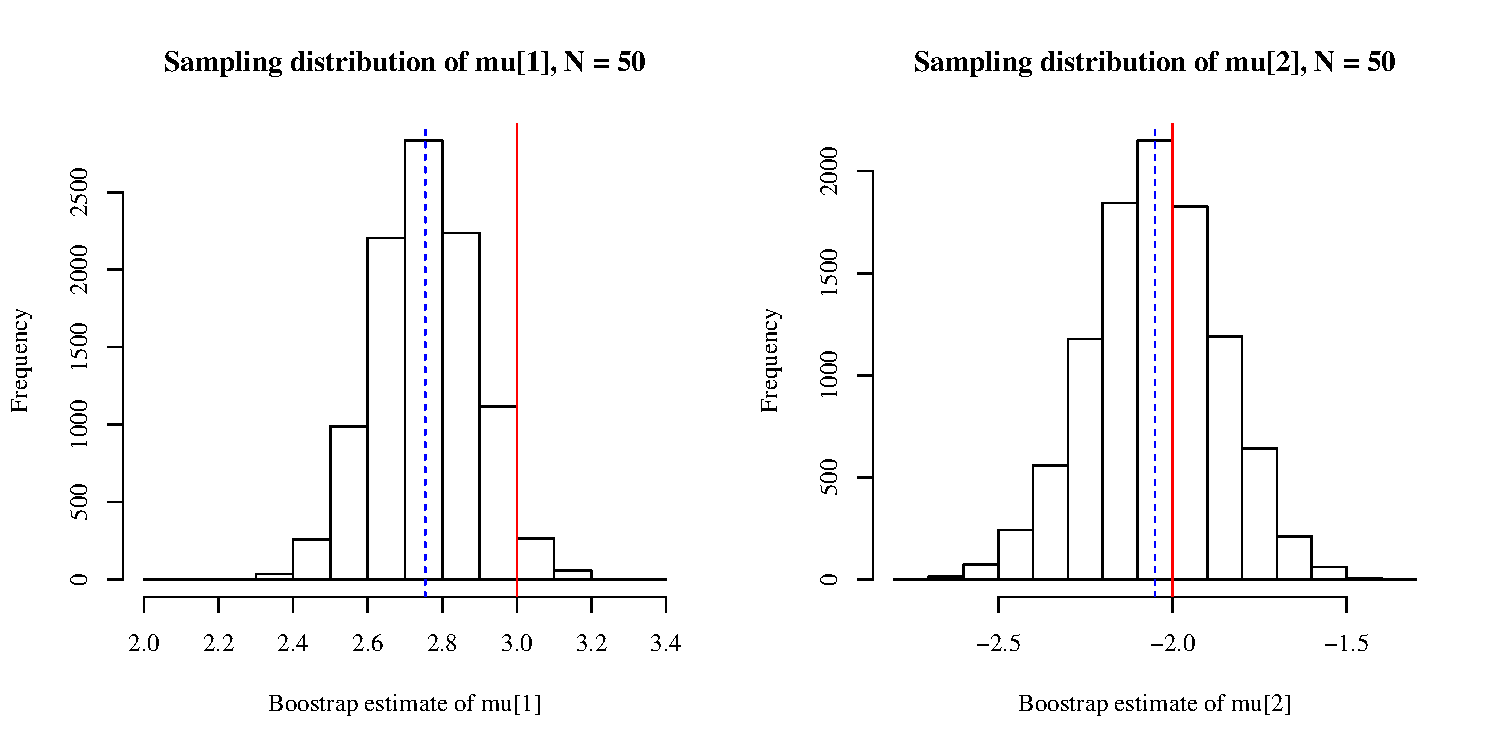
\includegraphics[scale=0.5]{mu.pdf}
			\caption{Estimated sampling distribution of mean vector}
			\label{fig:mufig}
		\end{figure}
		%
		%
		%
		\begin{figure}[htp!]
			\centering
				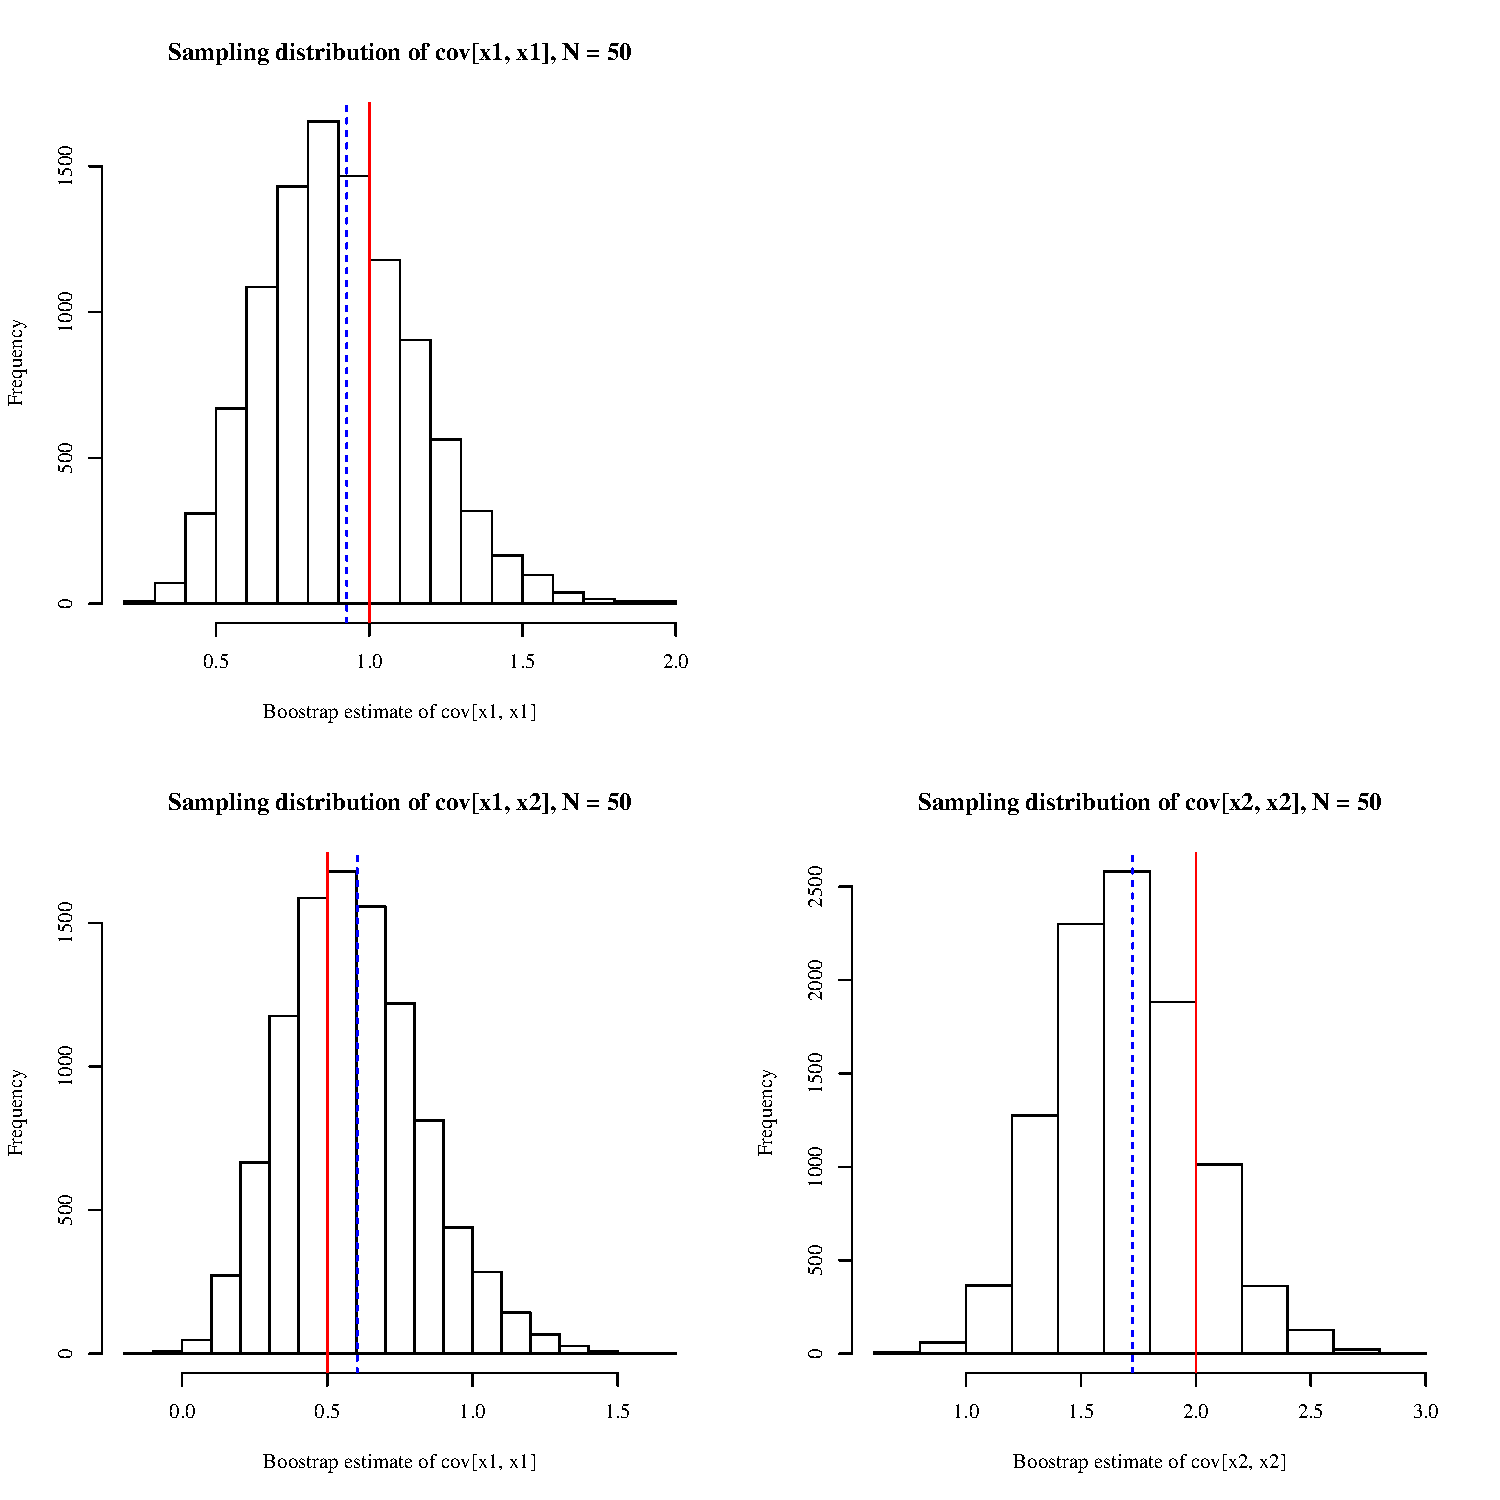
\includegraphics[scale=0.5]{Sigma.pdf}
			\caption{Estimated sampling distribution of covariance matrix}
			\label{fig:Sigmafig}
		\end{figure}
		%
		%
		%
	\end{enumerate}
	%
	%
	%
\end{enumerate}

\end{homeworkProblem}



%%----------------------------------------------------------------------------------------
%%	LIST CODE
%%----------------------------------------------------------------------------------------

\pagebreak
% \rscript{homework03.r}{Sample Perl Script With Highlighting}
R code for \texttt{myfuns.R}
\lstinputlisting[language=R]{myfuns.R}
\pagebreak
R code for \texttt{exercises01.R}
\lstinputlisting[language=R]{exercises01.R}


%----------------------------------------------------------------------------------------

\end{document}